% Section 6 (Entanglement as Spatial Information) mixes the ER=EPR discussion, the spatial bit concept, and the observer-relativity problem without fully resolving any of them. The sign puzzle paragraph is important and handled well, but the section as a whole feels like it's setting up future work more than delivering present results.
% 
% Claims that need tightening
% 
% The statement that the Unruh-Landauer relation and the Bekenstein bound "are the same inequality" (Section 2.4) is made confidently but the argument is essentially dimensional — you're substituting a=c2/Ra = c^2/R
% a=c2/R. The claim that "this appears to be new in this form" would benefit from a more careful literature check, particularly Bousso's work and Casini's reformulation of the Bekenstein bound.
% The EFT section (Section 8) makes the GHY term emergence argument, but the saddle point evaluation glosses over what it means to "integrate out the left wedge" in a non-perturbative sense. The double-counting argument for why SGHYS_{GHY}
% SGHY​ and SmatterLS_\text{matter}^L
% SmatterL​ aren't independent is physically intuitive but would benefit from being stated more carefully — a referee will push on this.
% Proposition 1 (EFT Validity) lists six equivalent conditions but the equivalences aren't all proven in the paper — some are asserted. Worth either proving them or labeling it as a conjecture/claim.
% 
% Missing pieces
% 
% You cite Wall's proof of the generalized second law but the connection to your single-microstate result deserves more discussion. Wall works in a different regime and a sentence noting why the classical focusing theorem suffices here (pure state, no need for QNEC) would help.
% The regularization appendix is good but you never discuss what happens to the BMS structure under regularization — you note the AS limit excites all BMS modes but the regulated case is left implicit.
% 
\documentclass[12pt,a4paper]{article}
\usepackage[width=.75\textwidth]{caption}
\usepackage{graphicx}
\usepackage{changepage}
\usepackage{authblk}
\usepackage{amsmath}
\usepackage{amsthm}
\usepackage{amsfonts}
\usepackage{amssymb}
\usepackage{braket}
\usepackage{enumerate}
\usepackage{etoolbox}
\usepackage{orcidlink}
\usepackage[mathscr]{euscript}
\usepackage[top=2cm, bottom=2cm, left=2cm, right=2cm]{geometry}
\usepackage{fancyhdr}
\usepackage{tikz-cd}
\newtheorem{prop}{Proposition}

\newcommand{\dv}[1]{\mathrm{d} #1 \text{ }}

\newcommand*\diff{\mathop{}\!\mathrm{d}}


\begin{document}


\title{Quantum Measurement, Minkowski Microstates and Matter Channels}
\author[ ]{Kevin Player\footnote{\textit{kjplaye@gmail.com}} \,\orcidlink{0009-0000-7180-7985}}

\maketitle

\abstract{
Thermodynamic approaches to gravity, from Jacobson to Verlinde, 
leave unspecified the microscopic carriers of individual entropy 
increments.
We show that the process of quantum measurement 
naturally models a gravitational microstate 
by developing an information-theoretic language 
of \emph{handoff events}, \emph{matter-memory}, 
and \emph{spatial bits}, in which matter and 
horizon are complementary timelike and spacelike 
channels.
Eliminating temperature 
between Landauer's principle and the Unruh effect yields an
acceleration-dependent bound on the energy associated with
information.
A single construction, a helicity-anticorrelated Bell state in flat
Minkowski space, makes contact with Jacobson's thermodynamic
derivation of the Einstein equations, Van Raamsdonk's entanglement-generated
geometry, the BMS supertranslation structure at horizons, a
Carnot cycle, and effective field theory.}


% Section 1
\section{Introduction}

We propose quantum measurement events as the elementary 
units of spacetime information processing and show this 
is consistent with geometric, thermodynamic, and effective 
field theory descriptions of the horizon. In this 
information-theoretic framework, matter is the fundamental 
substrate: proper time emerges from discrete action quanta 
accumulated along worldlines, spatial geometry emerges from 
handoff events at horizons, and the Planck area $\ell_P^2$ 
is the conversion factor between the two. This gives a 
Lorentz-invariant alternative to approaches that discretize 
geometry directly, discreteness lives in the matter 
sector via $\hbar$, and geometry inherits it through the 
covariant Raychaudhuri equation.

Thermodynamic approaches to gravity are remarkably successful 
and remarkably incomplete. Jacobson derives the Einstein 
equations from entropy and temperature on local Rindler 
horizons~\cite{jacobson1995thermodynamics}; Verlinde derives 
gravitational forces from entropy gradients on holographic 
screens~\cite{entropic}. Both frameworks operate at the level 
of bulk thermodynamics and neither specifies what physical 
process underlies each individual entropy increment. The 
information-theoretic framework proposed here supplies that 
process: quantum measurement events, modeled as energy-momentum 
transfers under proper acceleration, provide explicit 
realizations of those increments in flat Minkowski space.

The physical reasoning is as follows: any measurement is mediated by a physical 
interaction, so information acquisition necessarily involves an exchange of energy 
and momentum; by the equivalence principle, this impulse is locally 
indistinguishable from acceleration in a gravitational field. 
We do not claim to have a complete quantum gravity program; instead
we provide one explicit microstate construction, measurements of a
helicity-anticorrelated Bell state sourced by a bilocal 
term in flat Minkowski space, and situate it in the current literature.


\begin{figure}[h]
\centering
\begin{tikzcd}[row sep=4em, column sep=7em]
\text{Local Gravitational Effects} \arrow[r, dashed, "\scalebox{0.7}{\shortstack{Di\'osi--Penrose}}"]
    & \text{Quantum State Reduction} \\
\text{Acceleration} \arrow[u, "\scalebox{0.7}{\shortstack{local equivalence}}"']
                    \arrow[r, "\scalebox{0.7}{\shortstack{energy--momentum\\transfer}}"']
    & \text{Observation} \arrow[u, "\scalebox{0.7}{\shortstack{Bayesian\\update}}"']
\end{tikzcd}
\caption{Solid arrows denote subjective grounding relations 
for a given observer: $A \to B$ means every instance of $B$ 
is physically realised by an instance of $A$. This paper 
explores the solid arrows. The dashed 
arrow is the Di\'{o}si--Penrose postulate.}
\label{fig:diagram}
\end{figure}


That a single simple construction --- quantum measurement as energy--momentum 
transfer under proper acceleration, realised by one explicit photon pair in 
flat Minkowski space --- makes simultaneous contact with three independent 
programs suggests that measurement events of this kind may describe the 
elementary process those frameworks collectively require. We do not claim 
this construction is unique or irreducible; we claim it is sufficient and 
concrete.
Jacobson~\cite{jacobson1995thermodynamics} derives the Einstein 
equations from thermodynamic identities on local Rindler horizons but leaves 
open what physical process underlies each entropy increment at the level of 
individual microstates; the present paper proposes that process. 
Van~Raamsdonk~\cite{van2010building} showed, in the AdS/CFT setting, that 
entanglement between two spatial regions generates their geometric connection; 
the present construction realises the same effect in flat Minkowski space, 
microstate by microstate, with an explicit source. The BMS 
program~\cite{carlip2018black, hawking2016soft, strominger2016gravitational} 
identifies the symmetry algebra whose modes are excited at the horizon but does 
not specify what excites individual modes; the bilocal construction supplies 
a candidate process.

\subsection{Roadmap}

The central claim of this paper is the information-theoretic 
framework of Section~\ref{sec:substrate}: matter is the 
timelike substrate of emergent proper time, the horizon is 
the spacelike surface through which handoff events generate 
emergent space, and the Planck area $\ell_P^2$ is the 
conversion factor between the two descriptions. The 
event-by-event equality $S_{GHY}|_{\mathcal{H}} = 
S_{\mathrm{matter}}$, the Gibbons--Hawking--York boundary 
term and the matter action counting the same measurement 
events in geometric and informational language respectively,
is the consistency check that validates this framework. 
That it holds event by event rather than only at the 
thermodynamic ensemble level is what makes the check sharp: 
many microstructures are consistent with bulk thermodynamics, 
but the event-by-event equality constrains which ones are 
consistent with the geometry.

The paper has three layers. The \emph{framework layer} 
(Section~\ref{sec:substrate}) is the conceptual core: 
matter as a timelike information channel, the horizon as 
a spacelike handoff surface, and the handoff event as the 
elementary unit of both proper time and spatial geometry. 
This is the information-theoretic alternative to standard 
thermal quantum gravity that the rest of the paper 
elaborates and validates. The \emph{heuristic layer} 
(Section~\ref{sec:heuristics}) requires only Landauer's 
principle, the Unruh effect, and Newton's law; it recovers 
standard black hole thermodynamics from a temperature-free 
kinematic bound and is self-contained. The 
\emph{construction layer} 
(Sections~\ref{sec:microstates},~\ref{sec:ppwave}) 
exhibits one explicit Minkowski microstate, a Bell state 
of photons with anticorrelated helicities selected by a 
bilocal source, and shows that applying the Raychaudhuri 
equation to the resulting AS pp-wave yields 
$S_{GHY}|_{\mathcal{H}} = S_{\mathrm{matter}}$ event by 
event, consistent with the framework. 
Sections~\ref{sec:erepr}--\ref{sec:eft} apply the 
framework to entanglement-generated geometry, the 
equivalence of Carnot and Unruh--Landauer bounds, and 
the EFT origin of the GHY term.


% Section 2
\section{The Unruh--Landauer Bound and Motivating Heuristics}
\label{sec:heuristics}

Two structuring choices run throughout the paper. We work in the non-thermal 
global Minkowski description rather than the thermal Rindler description: 
thermality is a derived consequence of restricting to one 
wedge~\cite{fulling1973nonuniqueness, bisognano1975duality}, not a primitive, 
and individual microstates are non-thermal.

Our approach is a refactored version of the Di\'osi--Penrose objective collapse 
program~\cite{penrose1996gravity, diosi1987universal}, in the sense described
in the interpretational stance of Section~\ref{sec:introduction}: measurement 
is a subjective process mediated by energy--momentum transfer, with state 
reduction as a Bayesian update for a given observer grounded in common causal 
ancestry, as illustrated in Figure~\ref{fig:diagram}.

This section has two distinct parts. 
The Unruh--Landauer relation of 
Section~\ref{sec:UL} is an exact result 
that the construction layer inherits directly.
substituting the Unruh temperature into Landauer's bound 
eliminates temperature entirely, leaving a purely kinematic 
inequality depending only on acceleration. The subsequent 
derivations are explicitly Verlinde-style 
heuristics~\cite{entropic}: the same actors 
appear, acceleration, the Unruh relation, Newton's 
laws, but thermality is eliminated rather than embraced. 
Where Verlinde deploys the thermal Rindler frame as the 
mechanism connecting entropy to force, the Unruh--Landauer 
relation eliminates temperature entirely, and Newton's laws 
then recover standard black hole thermodynamics directly 
from the resulting kinematic bound. Thermality is a 
consequence of restricted causal access to one Rindler 
wedge~\cite{fulling1973nonuniqueness,bisognano1975duality}, 
not a primitive.

\subsection{The Unruh--Landauer Relation}
\label{sec:UL}


Landauer's principle~\cite{landauer1961irreversibility} 
establishes $k_BT$ as the natural energy scale of one 
distinguishable degree of freedom in a thermal environment 
at temperature $T$: any physical carrier representing 
$\Delta H$ nats must have at least this energy to be 
distinguishable from thermal noise,

\begin{equation}
  \Delta E \geq k_B T \, \Delta H.
\end{equation}

For an observer undergoing proper acceleration $a$, the Unruh effect associates a temperature
\begin{equation}
T = \frac{\hbar a}{2 \pi k_B c}
\end{equation}
with the local vacuum. Substituting into Landauer's bound eliminates $k_B T$, yielding
\begin{equation}
\boxed{\Delta E \geq \frac{\hbar a}{2\pi c} \, \Delta H.}
\label{eq:UL}
\end{equation}
Temperature has dropped out entirely: equation~\eqref{eq:UL} is a 
temperature-independent lower bound on the energy of the physical carrier 
required to register one nat of information under proper acceleration $a$; 
acceleration sets the minimum energy scale of the carrier. The full 
thermodynamic accounting, where the Landauer erasure cost appears,
is deferred to Section~\ref{sec:carnot}.


The connection between Landauer's principle and black hole 
thermodynamics has been noted previously. Cort\^{e}s and 
Liddle~\cite{cortes2024hawking} showed that Hawking 
evaporation saturates the Landauer bound at the Hawking 
temperature, identifying the two results as expressions of 
the same process at the level of bulk evaporation.
Related bounds on the energy cost of information 
acquisition in curved spacetime have been derived using 
the second law of thermodynamics applied to relativistic 
communication channels~\cite{alvim2024landauer}.
The present bound ~\eqref{eq:UL} differs in two respects: 
temperature is eliminated entirely by substituting the 
Unruh relation, yielding a purely kinematic bound depending 
only on acceleration, and the bound is applied to 
individual carrier quanta rather than to bulk evaporation. 

This Unruh--Landauer bound is saturated for a photon at one bit
when the wavelength equals the horizon distance up to a factor 
of $4\pi^2/\ln 2$:
\begin{equation}
\lambda_{\text{sat}} = \frac{4\pi^2}{\ln 2}\cdot\frac{c^2}{a} \sim d_{\mathcal{H}},
\end{equation}
where $d_{\mathcal{H}} = c^2/a$ is the proper distance to the 
Rindler horizon. The saturating photon is the fundamental mode of the causal diamond defined by the observer and the horizon, with wavelength commensurate with the horizon distance $d_\mathcal{H}$, too short to be 
super-horizon and too long to deposit more than one bit.
This identifies the horizon distance as the natural 
length scale of a single-bit measurement event, and 
the Rindler horizon as the surface at which the Landauer 
bound is geometrically realized.

For realistic accelerations the saturation wavelength is 
enormous, at Earth surface gravity $a = 9.8\ 
\text{m\,s}^{-2}$, $\lambda_{\text{sat}} \approx 8\ 
\text{light years}$, so the single-bit bound is 
practically always satisfied for terrestrial observers, 
and is only approached near astrophysical or Planck-scale 
accelerations.

\subsection{Momentum Transfer and Acceleration}
\label{sec:momentum}

\noindent\textbf{Note on method.}\; 
Sections~\ref{sec:momentum}--\ref{sec:bekenstein} 
are Verlinde-style dimensional analysis. They use 
Newtonian gravity and recover correct results at the 
Schwarzschild scale by the same coincidence exploited 
by Verlinde~\cite{entropic} and 
Bekenstein~\cite{bekenstein}: the Newtonian 
inverse-square law with a point mass reproduces the 
Schwarzschild geometry at the horizon scale, even 
though it formally breaks down there. This coincidence 
is specific to the spherically symmetric case; other 
matter distributions, including the bilocal source of 
Section~\ref{sec:microstates}, or the full Einstein 
equations, will in general give different results. 
The construction layer of 
Sections~\ref{sec:microstates}--\ref{sec:ppwave} 
makes no use of these heuristics. We make no attempt 
to disguise any of this.

\medskip

In what follows, standard results are 
\emph{reproduced as heuristic consequences} 
of the Unruh--Landauer relation and Newton's laws.
The energy transfer $\Delta E$ implied by the relation is carried by a physical quantum, matter or radiation,  mediating the measurement interaction as a \emph{thrust quantum}. For a relativistic carrier, the associated momentum transfer is
\begin{equation}
\Delta p = \frac{\Delta E}{c}.
\end{equation}
A measurement event localized to a spatial scale $r$ 
is bounded by a causal diamond with temporal extent 
$\Delta t = 2r/c$. This identification is the 
heuristic input from which the subsequent results 
follow, then

\begin{equation}
a = \frac{\Delta p}{m_d \Delta t} = \frac{\Delta E}{2 m_d r}.
\label{eq:accel}
\end{equation}

This is closely related to Verlinde's entropic 
gravity~\cite{entropic}: Verlinde identifies holographic 
thrust on information screens with the origin of inertia 
itself, and Newton's laws are a common ingredient in both 
constructions. The present approach differs in grounding 
each entropy increment in a discrete measurement event, the 
measurement impulse playing the role of Verlinde's 
holographic thrust, rather than in a coarse-grained 
thermodynamic gradient.


\subsection{The Schwarzschild Radius}

We match the kinematic acceleration of the detector to the 
gravitational field of the thrust quantum using Newton's laws. 
By $E = mc^2$, the energy quantum $\Delta E$ gravitates with 
effective mass $\Delta E / c^2$, producing a Newtonian 
gravitational acceleration
\begin{equation}
a = \frac{G \Delta E}{c^2 r^2}
\end{equation}
at distance $r$ from the detector. Equating this with the 
measurement-induced acceleration from equation~\eqref{eq:accel},
\begin{equation}
\frac{\Delta E}{2 m_d r} = \frac{G \Delta E}{c^2 r^2}.
\end{equation}
The energy $\Delta E$ of the thrust quantum cancels entirely: 
the Schwarzschild radius is independent of the energy of the 
carrier. Solving for $r$:
\begin{equation}
r = \frac{2 G m_d}{c^2} \equiv r_s,
\end{equation}
which is precisely the Schwarzschild radius of the detector 
mass $m_d$. The cancellation of $\Delta E$ is the physical 
content of the result: whatever energy the thrust quantum 
carries, the self-consistent horizon scale is set by the 
detector alone.

\subsection{Surface Gravity}
Evaluating the acceleration at $r = r_s$ gives the surface gravity of the detector:
\begin{equation}
\kappa = \frac{G m_d}{r_s^2} = \frac{c^4}{4 G m_d},
\end{equation}
in agreement with the standard Schwarzschild result, 
as expected from the Verlinde coincidence. This 
reproduces the acceleration appearing in the Unruh 
temperature $T = \hbar \kappa / 2\pi k_B c$, 
providing an internal consistency check on the 
heuristics.

\subsection{Bekenstein--Hawking Entropy}
\label{sec:bekenstein}

Returning to the Unruh-Landauer relation~\eqref{eq:UL} and 
substituting the surface gravity $\kappa$ for $a$, justified 
by the equivalence principle: the local quantum field theory at 
the black hole horizon is the same as in the Rindler 
frame~\cite{unruh1976notes, hawking1975particle}, the entropy 
increment associated with an energy increment 
$\Delta E = c^2 \Delta m_d$ is

\begin{equation}
\Delta H \leq \frac{2\pi c}{\hbar \kappa} \Delta E = \frac{8\pi G m_d}{\hbar c^3} \cdot \Delta m_d c^2.
\end{equation}
Expressing this in terms of the change in Schwarzschild area $\Delta A = 32\pi G^2 m_d \Delta m_d / c^4$:
\begin{equation}
\Delta H \le \frac{\Delta A}{4 \ell_P^2}, \qquad \ell_P^2 = \frac{\hbar G}{c^3},
\end{equation}
which is the Bekenstein-Hawking area law. Each measurement event contributes a discrete entropy increment proportional to the area imprinted on the horizon by the associated energy-momentum transfer.

This derivation parallels Jacob Bekenstein’s original argument \cite{bekenstein}, in which the entropy increase of a black hole is inferred from the minimal energy required to localize and drop a system across the horizon; here, the same structure emerges from the minimal energy cost of registering information at the horizon scale.

The two bounds are saturated simultaneously when $a = c^2/R$ — which is exactly the condition for being {\it at a horizon}. The horizon is therefore not just where thermodynamics happens to work out, it is the unique locus where the minimum cost of information acquisition equals the maximum information content of the region.

Substituting the horizon condition $a = c^2/R$ directly 
into the Unruh--Landauer bound~\eqref{eq:UL} yields
\begin{equation}
    \Delta H \leq \frac{2\pi R\,\Delta E}{\hbar c},
\end{equation}
which is precisely the Bekenstein universal entropy 
bound~\cite{bekenstein1981universal} on the 
entropy-to-energy ratio for a system of size $R$. 
The Unruh--Landauer relation and the Bekenstein bound 
are therefore the same inequality: the former is its 
acceleration-frame expression, the latter its 
position-space expression, and the Rindler horizon is 
the surface at which the two descriptions coincide.
The covariant generalisation of the Bekenstein bound to arbitrary null 
hypersurfaces is the Bousso bound~\cite{bousso1999covariant}, which 
bounds entropy on any non-expanding null congruence by the area of its 
generating surface. The Raychaudhuri derivation of 
Section~\ref{sec:ppwave} operates precisely on such a congruence; the 
present construction can be read as a microstate-level realisation of the Bousso bound, with each handoff event contributing one Planck-area patch to the light-sheet.


Pesci~\cite{pesci2007unruh} derived the covariant entropy bound from the 
Unruh temperature by applying the second law of thermodynamics across 
local Rindler horizons, the closest precursor to the present argument. 
The present bound equation~\eqref{eq:UL} differs in two respects: temperature is 
eliminated entirely by substituting the Unruh relation into Landauer's 
principle rather than retained as an input to the second law, yielding a 
purely kinematic bound depending only on acceleration; and the bound is 
applied to individual carrier quanta rather than to a bulk thermodynamic 
flux. The identification of equation~\eqref{eq:UL} with the Bekenstein 
bound~\cite{bekenstein1981universal} at the horizon condition $a = c^2/R$, 
and the reading of both as the same inequality in different frames, 
appears to be new in this form.

% Section 3
\section{Bilocal Microstate Construction}
\label{sec:microstates}

From now on we use natural units $\hbar = c = 1$ unless 
otherwise specified; factors of $\hbar$ and $c$ are restored 
where they aid physical interpretation.

The arguments of Section~\ref{sec:heuristics} motivate a 
heuristic relationship between information acquisition, 
acceleration, and gravitational effects, but leave open the 
question of what a single microstate looks like concretely. 
In standard treatments, the Unruh effect is derived by 
coupling a detector to a pre-existing acceleration and reading 
off a thermal response from the vacuum. 
In~\cite{player2025driving} this logic was inverted for a 
scalar field: a source placed in the past injects non-thermal 
entangled excitations into the field, and the observer's 
accelerated response was shown to be driveable by these 
source-induced excitations. We extend that construction here 
to the spin-1 electromagnetic field, upgrading from scalar 
to helicity-carrying Bell states and making the single-bit 
structure of each measurement event explicit.

A \emph{Minkowski microstate} is, in this paper, a single 
explicit quantum event in flat Minkowski space, a 
photon pair emitted by a physical source, detected by 
two accelerated observers, that realises one discrete 
entropy increment of the kind that Jacobson and Verlinde 
require at the thermodynamic level. We make no claim that 
this is the unique such construction; other configurations, 
with back-reaction, asymmetric detector placement, or 
different source geometries, would also qualify. The 
construction below is simply the smallest one we could 
exhibit that is clean enough to track consistently through 
the geometric, thermodynamic, information-theoretic, and 
effective field theory frameworks simultaneously.

\subsection{A Source and Two Observers}

Three massive bodies are placed at spacetime positions 
$(t,z) = (0,1)$, $(0,-1)$, and $(-1,0)$, named 
\emph{$\mathcal{R}$}~--~\textit{Right}, 
\emph{$\mathcal{L}$}~--~\textit{Left}, and 
\emph{$\mathcal{P}$}~--~\textit{Past} respectively. 
$\mathcal{P}$ serves as the common causal ancestor of the 
accelerations of $\mathcal{R}$ and $\mathcal{L}$ (see 
Figure~\ref{paz}). $\mathcal{P}$ emits an entangled pair of 
spin-1 massless photons with momenta $\pm k$ and Rindler 
frequency $\omega = \omega_k$.
The momenta are perfectly balanced by construction: the two photons 
carry spatial momenta $+k\hat{z}$ and $-k\hat{z}$ respectively, so 
the total linear momentum vanishes, $k + (-k) = 0$. The angular 
momentum vanishes term by term: in each helicity assignment 
$(\lambda_R, \lambda_L) = (+1,-1)$ and $(-1,+1)$, the total 
helicity is $\lambda_R + \lambda_L = (+1) + (-1) = 0$ and 
$(-1) + (+1) = 0$ respectively, and the symmetric Bell state 
superposition~\eqref{eq:microstate_vec} preserves this since 
both terms contribute zero independently. The source therefore 
exhibits no net back-reaction in either linear or angular momentum.
The two photons propagate into the left and right Rindler wedges, 
where $\mathcal{L}$ and $\mathcal{R}$ detect them respectively 
via absorption, the momentum impulse of which accelerates each 
detector into its respective Rindler wedge; each observer thereby 
registers a helicity eigenvalue and acquires one classical bit 
of information.
The emission event at $\mathcal{P}$ naturally defines 
null coordinates $u = t - z + 1$ and $v = t + z + 1$, 
centered so that $\mathcal{P}$ lies at $u = v = 0$, 
the right-moving photon propagates along $u = 0$, 
and the left-moving photon propagates along $v = 0$.

\begin{figure}[h]
\centering
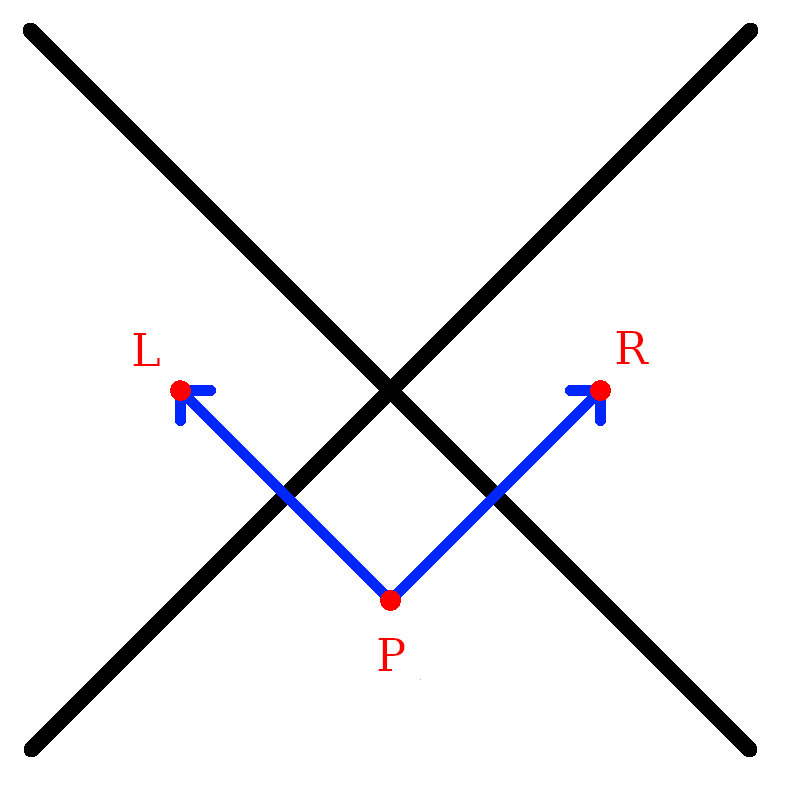
\includegraphics[scale=0.75]{paz.png}
\captionsetup{width=0.7\textwidth}
\caption{A source in the past, $\mathcal{P}$, emits an 
entangled photon pair that accelerates $\mathcal{R}$ into 
the right Rindler wedge and $\mathcal{L}$ into the left 
Rindler wedge.
The two null directions of propagation define 
the null coordinates $u = t - z + 1$ and $v = t + z + 1$, 
with the right-moving photon propagating along $u = 0$ 
and the left-moving photon along $v = 0$; these are 
the $z^-$ and $z^+$ axes of the double-null coordinate 
system of Section~\ref{sec:doublenull}.}
\label{paz}
\end{figure}

The three-party structure $\mathcal{P}$--$\mathcal{R}$--$\mathcal{L}$ 
realises a form of tripartite entanglement with a natural 
interior reconstruction interpretation. 
Neither $\mathcal{R}$ nor $\mathcal{L}$ alone can distinguish 
a correlated Bell-state emission at $\mathcal{P}$ from an 
uncorrelated thermal source: each observer's reduced 
density matrix is thermal, exactly as in the standard Unruh 
effect. Together, their two anticorrelated bits reveal the 
correlation structure of the emission event, identifying it 
as a specific Bell state at a specific frequency, and 
providing a microstate-level analogue of black hole 
interior reconstruction~\cite{penington2020entanglement, 
almheiri2021entropy}, where the interior is recovered 
as classical correlations in the joint record of 
complementary exterior observers.

\subsection{PVM Localization and the Elimination of Coarse-Graining}
\label{sec:pvm_localization}

The Unruh mode plays a double role in this
construction. As a QFT object it is a coefficient in a mode expansion, 
a solution to the wave equation analytically continued 
from the Rindler wedge into all of Minkowski space. 
But once $\mathcal{P}$ is specified as a real physical 
source via the squeezing interaction~\eqref{eq:bilocal_lag}, 
the mode function acquires a second interpretation: 
it is a probability amplitude in the Born rule sense, 
encoding where $\mathcal{R}$ is likely to detect the 
emitted quantum. This is the inversion of the standard 
Unruh--DeWitt logic. Rather than coupling a detector to 
a pre-existing acceleration and reading off a thermal 
distribution by averaging over all Rindler frequencies, 
we front-load the logic at $\mathcal{P}$: the source 
fixes the frequency $\omega_k$ and the mode function 
then specifies the probability amplitude for detection. 

Thermality, in this picture, is not a primitive 
property of the vacuum seen by an accelerating observer 
but a consequence of residual ignorance, about the 
precise location of $\mathcal{R}$ within the wedge, 
and about the spatial origin of the detected excitation, 
that the present construction resolves by specifying 
the common causal ancestry of $\mathcal{P}$, 
$\mathcal{R}$, and $\mathcal{L}$ explicitly. The 
ignorance is epistemic, not ontic: the global Minkowski 
state remains pure throughout, and thermality is what 
a single-wedge observer sees when causal access to 
$\mathcal{P}$'s emission event is unavailable.

\begin{figure}[h]
\centering
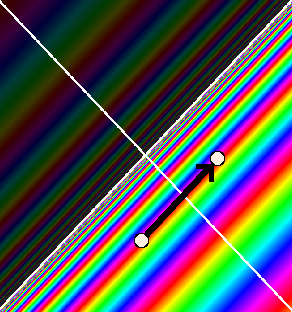
\includegraphics[scale=0.5]{paz_freq.png}
\captionsetup{width=0.7\textwidth}
\caption{The points $\mathcal{P}$ and $\mathcal{R}$ are marked 
with white dots, connected by the null geodesic (black arrow). 
The rainbow coloring shows the Unruh mode phase 
structure across Minkowski space. A PVM projection onto this null line selects 
a single frequency from the thermal superposition, replacing 
the full delocalized mode with the localized non-thermal 
microstate of equation~\eqref{eq:microstate_vec}.}
\label{paz_freq}
\end{figure}

This inversion has a geometric consequence that 
runs through the entire paper: it is precisely what 
allows the construction to live in flat Minkowski 
space rather than requiring an AdS/CFT dual. In the 
standard holographic picture, geometry is primary 
and entanglement is read off it, Van 
Raamsdonk's argument~\cite{van2010building} proceeds 
from the entanglement entropy of a boundary state to 
the geometry of the bulk ER bridge.


Here the direction of explanation is reversed: the 
emission event at $\mathcal{P}$ is primary, and the 
geometry,the AS pp-wave, the horizon area increment, 
the BMS supertranslation, is the \emph{ontic} output 
of the subsequent measurement events at $\mathcal{R}$ 
and $\mathcal{L}$. The geometry is a real physical 
change; what is epistemic is the assignment of that 
change to a particular observer's microstate record. 
These are distinct, and keeping them distinct is what 
allows the construction to live in flat Minkowski space 
without a holographic dual.

\paragraph{Longitudinal localization.}
The primary localization is in the longitudinal $(t,z)$ 
plane, which is the setting of Figure~\ref{paz_freq} 
and of the parabolic cylinder function analysis 
of~\cite{player2025driving}.
In that work, a Minkowski mode $\varphi_q^*$ multiplied 
pointwise by a Gaussian shaping function $N_{\mu,\sigma}$ 
of width $\sigma$ in $(t,z)$, then paired via the 
Klein--Gordon inner product with a Rindler mode $r_k$, 
yields an overlap expressible in terms of parabolic 
cylinder functions $D_\nu(-\zeta)$. The Gaussian could 
equivalently have been applied to the Rindler side; 
what matters is that $\sigma$ controls the degree of 
longitudinal localization of the source-detector pair.
The Stokes phenomenon 
in the asymptotics of $D_\nu(-\zeta)$ as $\sigma$ varies 
drives a transition between two physically distinct 
regimes: $\sigma \to \infty$ gives the thermal regime 
where the $e^{-\frac{1}{4}\zeta^2}$ branch dominates, 
and $\sigma \to 0$ gives the localized non-thermal 
regime where the $e^{+\frac{1}{4}\zeta^2}$ branch dominates, 
with the Stokes line at $\arg \zeta = \pi/4$ marking the 
boundary between them.

In the present paper the same Gaussian shaping function 
is reread as a Kraus operator acting on the quantum state.
\begin{equation}
  K_\sigma = \int e^{-u^2/2\sigma^2}\;
|u\rangle\langle u|\; du,
\label{eq:kraus_longitudinal}
\end{equation}
where $u = t - z + 1$ is the null coordinate\footnote{We use $\zeta$ for the Stokes variable 
of~\cite{player2025driving} to avoid confusion 
with the longitudinal spatial coordinate $z$.}
defined in Section~\ref{sec:ppwave}.
The operator $K_\sigma$ together with its complement 
\begin{equation}
K_\sigma^\perp = \int \sqrt{1 - e^{-u^2/\sigma^2}}\;
|u\rangle\langle u|\; du,
\end{equation}
satisfying 
$K_\sigma^\dagger K_\sigma + 
(K_\sigma^\perp)^\dagger K_\sigma^\perp = \mathbf{1}$ 
by construction, defines a one-parameter POVM family;
the Stokes transition between its two asymptotic 
regimes is illustrated in Figure~\ref{stokes_kraus}.
Specifying $\mathcal{R} = (0,1)$ 
and $\mathcal{P} = (-1,0)$ is precisely the $\sigma \to 0$ 
limit: the Kraus operator sharpens to a PVM projector 
onto the unique null geodesic connecting them, selecting 
a single definite frequency $\omega_k$ from what would 
otherwise be a thermal superposition over all Rindler 
frequencies. This is visible directly in 
Figure~\ref{paz_freq}: the rainbow phase structure of 
the Unruh mode concentrates onto the null line between 
$\mathcal{P}$ and $\mathcal{R}$, and the PVM projection 
selects that line. The Stokes transition 
of~\cite{player2025driving} is therefore not merely a 
field-theoretic regularization result but the analytic 
signature of the POVM-to-PVM transition: the same 
mathematical object is being read in two complementary 
languages, field theory and measurement theory, with 
the Stokes line marking the boundary between them.
The helicity label $\lambda$ enters the longitudinal 
mode function as a spectator index and does not affect 
the $u$-dependence of the Kraus 
operator~\eqref{eq:kraus_longitudinal}; the Stokes 
transition analysis of~\cite{player2025driving} therefore 
applies independently to each helicity sector without 
modification.

\begin{figure}[h]
\centering
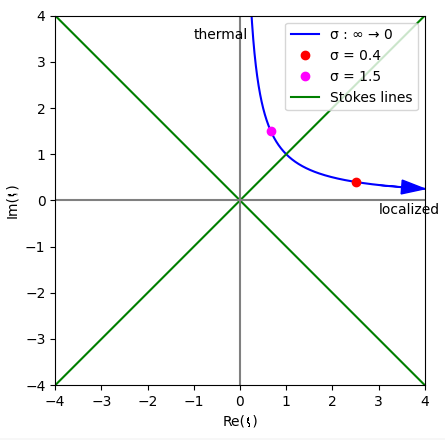
\includegraphics[scale=0.5]{stokes.png}
\captionsetup{width=0.7\textwidth}
\caption{
Trajectory of $\zeta = iq\sigma + \mu/\sigma$ 
in the complex plane as $\sigma$ interpolates 
between the two limits of the Kraus 
family~\eqref{eq:kraus_longitudinal}. The thermal limit 
$\sigma \to \infty$ corresponds to $\zeta$ on the 
positive imaginary axis; the localized PVM limit 
$\sigma \to 0$ corresponds to $\zeta$ on the positive 
real axis. The green Stokes lines at 
$\arg \zeta = \pi/4$ mark the boundary between the 
two asymptotic regimes of the parabolic cylinder 
function $D_\nu(-\zeta)$, and therefore the boundary 
between the POVM and PVM descriptions of the 
longitudinal localization. Figure 
from~\cite{player2025driving}.}
\label{stokes_kraus}
\end{figure}

\paragraph{Transverse localization.}
The transverse $(x,y)$ directions require a separate 
and independent localization.
A Rindler plane wave at frequency $\omega$ is a coherent 
superposition over all possible source-detector pairs 
$(\mathcal{P}', \mathcal{R}')$ connected by null geodesics 
at that frequency, uniform in the transverse plane. 
The longitudinal and transverse localizations decouple 
because the wave equation in double-null coordinates 
separates: the $u$-dependence and the $(x,y)$-dependence 
of the mode function enter independently, so the two 
Kraus projections can be applied in either order without 
interference.
Specifying 
$\mathcal{P} = (-1,0)$ and $\mathcal{R} = (0,1)$ 
performs a second PVM projection, now in the transverse 
directions, selecting the unique null geodesic and 
resolving the remaining coarse-graining over transverse 
position. The transverse shaping is controlled by an 
independent width $\sigma_\perp$, which we treat as a 
free parameter in Section~\ref{sec:two_regimes} and 
whose physical consequences are developed in 
Section~\ref{sec:ppwave}.

The two widths $\sigma$ and $\sigma_\perp$ control 
physically distinct aspects of the construction and 
need not be sent to zero together. The longitudinal 
$\sigma$ governs the POVM-to-PVM transition and the 
thermal-to-non-thermal transition analyzed via the 
Stokes phenomenon; Section~\ref{sec:microstates} 
works entirely in the $\sigma \to 0$ PVM limit. 
The transverse $\sigma_\perp$ controls the spatial 
profile of the horizon perturbation and the BMS mode 
content: $\sigma_\perp \to \infty$ produces a planar 
impulsive wave exciting a single BMS supertranslation 
mode, while $\sigma_\perp \to 0$ recovers the 
Aichelburg--Sexl pp-wave with logarithmic shift 
$\Delta v \propto -\ln r^2$ exciting the full BMS 
spectrum. The area increment $\Delta A = 8\pi G\hbar\omega$ and 
the event-by-event equality 
$S_{GHY}|_{\mathcal{H}} = S_{\mathrm{matter}}$, 
which serve as the geometric consistency checks of 
the framework, are independent of $\sigma_\perp$, 
fixed by energy conservation alone.

\paragraph{The microstate.}
The result of both projections is an individually 
non-thermal microstate carrying a definite Rindler 
frequency $\omega$ and a definite longitudinal 
position on the null geodesic from $\mathcal{P}$ 
to $\mathcal{R}$. Thermality is not a property of 
any single microstate but of the ensemble; it 
emerges when one models the detector response 
within a wedge as a sum over all Rindler modes, 
as in the standard Unruh--DeWitt 
treatment~\cite{unruh1976notes,einstein1979general}, 
and is a consequence of that mode-averaging rather 
than a premise of the construction. The individual 
non-thermal microstate is what the PVM projection 
onto the $\mathcal{P}$--$\mathcal{R}$ null geodesic 
selects; the thermal ensemble is what remains when 
neither coarse-graining is resolved and $\mathcal{L}$ 
is traced out.

A note on the $\sigma \to 0$ idealization: throughout 
this paper the PVM limit is understood as the 
idealization of a physical construction that lives 
at small but finite $\sigma$. At exactly $\sigma = 0$ 
the Kraus operator~\eqref{eq:kraus_longitudinal} 
becomes a projector onto a set of measure zero in 
the continuum $|u\rangle$ basis and is no longer 
normalizable in the strict sense; similarly, the 
AS longitudinal shift $\Delta v \propto -\ln r^2$ 
diverges on axis at $r = 0$ in the strict localized 
limit. Both divergences are regularized by keeping 
$\sigma > 0$, as carried out explicitly for the 
geometric side in Appendix~\ref{sec:as_reg}. The 
parameter $\sigma$ therefore plays a unified role: 
it is simultaneously the width of the Kraus operator 
in the longitudinal direction, the transverse profile 
width of the photon mode, and the regularization 
scale of the AS singularity, all controlled by the 
same physical quantity, the photon wavelength 
$\sigma \sim c/\omega$. All sharp statements about 
individual microstates should be understood as 
holding in the limit $\sigma \to 0^+$ rather than 
at exactly $\sigma = 0$.



\subsection{Helicity Structure and PCT Symmetry}

We now upgrade this construction from a spin-0 scalar field 
in~\cite{player2025driving} to the spin-1 electromagnetic 
field with a superposition of helicity pairs in a Bell state, 
introducing one unknown binary degree of freedom,  the 
helicity outcome, undetermined until measured,  which is 
the single bit responsible for the remaining thermality in 
the ensemble. The photon carries one quantum of action $\hbar$ 
and energy $E = \hbar\omega$, identifying the thrust quantum 
of Section~\ref{sec:heuristics} with a single photon whose 
polarization outcome, upon detection, is the classical bit 
acquired by each observer. The Bell state is the natural 
completion of the PCT symmetry between wedges, which by the 
Bisognano--Wichmann theorem~\cite{bisognano1975duality} is 
implemented by the modular conjugation operator $J$ mapping 
the right wedge algebra to the left wedge algebra, and as we 
discuss in Section~\ref{sec:ppwave}, the photons imprint a 
definite geometric signature onto the horizon.


The anticorrelated helicity assignment traces to the PCT 
symmetry implemented by the Bisognano--Wichmann modular 
conjugation $J$, which maps the right-wedge algebra to the 
left-wedge algebra and simultaneously flips $\lambda \to 
-\lambda$; the Bell state~\eqref{eq:microstate_vec} is the 
natural state in this momentum sector invariant under that 
operation. The common algebraic origin of this anticorrelation 
in the Lorentz algebra decomposition $\mathfrak{so}(3,1) \cong 
\mathfrak{su}(2) \times \mathfrak{su}(2)$, and its connection 
to the ``tick-tock'' mechanism of Section~\ref{sec:zigzag}, is 
developed in detail in Section~\ref{sec:zigzag}.

\subsection{Double-Null Gauge}
\label{sec:doublenull}
The emission event naturally defines two null directions: the 
right-moving photon has wave-vector 
$k^\mu_R = (\omega, 0, 0, k)$ and the left-moving photon has 
wave-vector $k^\mu_L = (\omega, 0, 0, -k)$, with equal and 
opposite spatial momenta. These two null directions are 
precisely the $z^+$ and $z^-$ axes of double-null coordinates
\begin{equation}
  z^\pm = \frac{1}{\sqrt{2}}(t \pm z) 
  = \frac{1}{\sqrt{2}}(u - 1 \pm (v - 1)),
\end{equation}
with transverse coordinates $\mathbf{z}_\perp = (x, y)$. 
Note that $z^\pm$ are centered on the Minkowski origin 
$(t,z) = (0,0)$ rather than on $\mathcal{P}$; the 
coordinates $u, v$ defined in 
Section~\ref{sec:microstates} are the $\mathcal{P}$-centered 
versions and are used throughout the remainder of the paper.
Working in this frame we impose the symmetric double-null 
gauge condition
\begin{equation}
    A_+(z) = 0, \qquad A_-(z) = 0,
\label{eq:doublenull}
\end{equation}
so that the gauge field is supported entirely on the 
transverse components $\mathbf{A}_\perp = (A^x, A^y)$. This 
gauge respects the PCT symmetry that swaps the two wedges 
$(z^+ \leftrightarrow z^-)$ simultaneously with 
$(R \leftrightarrow L)$, and therefore treats both observers 
symmetrically by construction. The residual gauge freedom is 
fixed by requiring $\partial_i A^i = 0$ in the transverse 
plane, leaving precisely the two physical helicity degrees of 
freedom $\epsilon^i_{(\lambda)}$ with $\lambda = \pm 1$; 
consistency with Maxwell's equations and the absence of 
over-determination are verified in 
Appendix~\ref{gauge_consistency}.

The lack of manifest four-dimensional covariance in 
equation~\eqref{eq:doublenull} is a consequence of aligning 
the gauge with the pair of physical null directions selected 
by the source, rather than an arbitrary choice. The full 
Lorentz group is broken to the little group preserving the 
pair $\{k^\mu_R, k^\mu_L\}$, which is the two-dimensional 
Euclidean group $ISO(2)$ acting on the transverse plane. This 
is precisely the little group of massless particles, and the 
two helicity eigenstates $\lambda = \pm 1$ are its 
irreducible representations. All physical results are independent of the gauge choice: 
the helicity eigenvalues $\lambda = \pm 1$ are representations 
of the massless little group $ISO(2)$ and are therefore 
Poincar\'{e}-covariant objects independent of how the 
gauge is fixed, and the consistency of the double-null 
gauge with Maxwell's equations and the correct degree-of-freedom 
count is verified explicitly in Appendix~\ref{gauge_consistency}.

\subsection{The Bilocal Source}

In double-null gauge the electromagnetic field is 
characterised by its transverse components alone. The bilocal 
driving source is symmetrized over both helicity assignments,
\begin{equation}
    J^{ij}(x,y) = g\left( \epsilon^{i*}_{(-1)}\, 
    \epsilon^{j}_{(+1)} 
    + \epsilon^{i*}_{(+1)}\, \epsilon^{j}_{(-1)}\right) 
    f_L(x)\, f_R(y),
\label{eq:bilocal_vec}
\end{equation}
where $f_L$ and $f_R$ are normalised mode profiles 
supported on the left and right wedges respectively, 
and $\epsilon^i_{(\lambda)}$ are the circular 
polarization vectors
\begin{equation}
    \epsilon^i_{(+1)} = \frac{1}{\sqrt{2}}
    \begin{pmatrix}1\\i\end{pmatrix}, \qquad
    \epsilon^i_{(-1)} = \frac{1}{\sqrt{2}}
    \begin{pmatrix}1\\-i\end{pmatrix}.
\end{equation}
The two terms in~\eqref{eq:bilocal_vec} are related by the 
PCT transformation in the sense of 
Bisognano--Wichmann~\cite{bisognano1975duality}, which maps 
the right wedge algebra to the left wedge algebra and 
simultaneously flips $\lambda \to -\lambda$.

More precisely, the modular conjugation $J$ of 
Bisognano--Wichmann maps a right-wedge creation operator 
$a^{R\dagger}_{k,(\lambda)}$ to a left-wedge creation 
operator $a^{L\dagger}_{-k,(-\lambda)}$, implementing PCT 
between wedges. The Bell state~\eqref{eq:microstate_vec} is a natural 
two-photon state at fixed frequency $\omega$ and fixed 
momentum pair $(k, -k)$, invariant under $J$: within
this momentum sector, 
the anticorrelated helicity assignment and the symmetric 
superposition are not choices but consequences of requiring 
$J$-invariance, since $J$ flips both helicity and wedge 
simultaneously, leaving no room for a relative phase or 
helicity-correlated alternative.
The bilocal source~\eqref{eq:bilocal_vec} is therefore 
a natural source, consistent with the algebraic symmetry 
of the Rindler vacuum, and the simplest one we could 
construct with the required properties.

The symmetrization is consistent with PCT symmetry and 
angular momentum conservation at the emission vertex. 
Other source geometries are possible; this one is chosen 
for its simplicity and the transparency of its connection 
to the algebraic structure of the Rindler vacuum. The argument 
has three steps. First, a scalar source carries zero angular 
momentum, so the emitted pair must satisfy $\lambda_R + 
\lambda_L = 0$, which forces the two helicities to be 
anticorrelated: the only possibilities are $(\lambda_R, 
\lambda_L) = (+1,-1)$ or $(-1,+1)$. Second, the Bisognano--Wichmann 
modular conjugation $J$ maps the first assignment to the 
second and vice versa, so the unique $J$-invariant state in 
this sector is their symmetric superposition with relative 
phase fixed by $J$-invariance. Third, any other relative 
phase or asymmetric combination would break the PCT symmetry 
between wedges, which is a symmetry of the Minkowski vacuum 
and must therefore be preserved by the source. The total 
angular momentum vanishes in both terms independently.

The bilocal source selects a specific microstate from 
the Minkowski vacuum by a PVM projection onto the $n=1$ 
sector at fixed $\omega$ and fixed helicity pair 
$(\lambda, -\lambda)$, in exact analogy with the scalar 
construction of~\cite{player2025driving}. No perturbative 
expansion in a coupling constant is required: the 
helicity-anticorrelated photon pair is already present 
in the vacuum decomposition~\eqref{eq:vacuum_vec}, and 
the bilocal source selects it via the PVM projection of 
Section~\ref{sec:pvm_localization}. The operator content 
of this selection is
\begin{equation}
        a^{L\dagger}_{-k,(-1)}\, a^{R\dagger}_{k,(+1)}
          \;+\;
          a^{L\dagger}_{-k,(+1)}\, a^{R\dagger}_{k,(-1)}
          \;+\;
          \text{h.c.},
\label{eq:bilocal_lag}
\end{equation}
where the two creation operator pairs correspond to the 
two PCT-related helicity assignments, each carrying total 
angular momentum zero, consistent with emission from a 
scalar source at $\mathcal{P}$. This is the vector-field 
analogue of the scalar squeezing 
interaction~\cite{gerry2023introductory}, with the PCT 
symmetry between wedges made explicit; the connection to 
the quantum optics squeezing literature is structural 
rather than perturbative.

Each photon carries energy $E = \hbar\omega$ and one quantum 
of action $\hbar$, identifying the thrust quantum of 
Section~\ref{sec:heuristics} with a concrete physical object: 
the minimum actionable event is precisely a single photon. 
Its polarization, undetermined until measured, is the quantum 
bit whose outcome constitutes the classical record acquired by 
each observer upon detection.

The Unruh--Landauer bound is saturated not at the level of an 
individual photon but at the level of the source rate. The 
acceleration $a$ does not fix the frequency $\omega$ of each 
selected quantum; rather, it determines the rate $\dot{N}$ at 
which the bilocal source selects entangled pairs in order to 
implement that acceleration, with the total power 
$\dot{N}\hbar\omega$ matching the Unruh thermal flux.
Each individual photon carries exactly one quantum of action 
$\hbar$ and one binary helicity outcome, one bit in the sense 
of one binary alternative carrying $\ln 2$ nats, and these 
are paired by the construction independently of $a$. The 
Landauer bound then operates as a consistency condition on 
the ensemble: the minimum energy cost per bit acquired, 
summed over the rate of acquisition, equals the power 
required to sustain the acceleration.

\subsection{Polarization Bogoliubov Transformation}

We now show that the polarization labels survive the 
Rindler--Unruh mode decomposition, so that the thermal 
ensemble retains its helicity structure and the 
anticorrelation of the emitted pair descends unambiguously 
to the level of individual Rindler microstates.

In the transverse plane, the electromagnetic field in 
double-null gauge decomposes into two independent 
scalar-like sectors labelled by helicity $\lambda = \pm 1$. 
For each sector, the right-wedge field expands as
\begin{equation}
    A^i_\lambda(z) = \int_0^\infty \frac{d\omega}{2\pi}\,
        \frac{1}{\sqrt{2\omega}}\,\epsilon^i_{(\lambda)}
        \left[
            b^R_{\omega,\lambda}\, u^R_\omega(z)
            + b^{R\dagger}_{\omega,\lambda}\, u^{R*}_\omega(z)
        \right],
\end{equation}
where $u^R_\omega(z)$ are the right-wedge Rindler modes at 
Rindler frequency $\omega$, and $b^R_{\omega,\lambda}$, 
$b^{R\dagger}_{\omega,\lambda}$ are the corresponding 
annihilation and creation operators satisfying
\begin{equation}
    \left[b^R_{\omega,\lambda},\, 
    b^{R\dagger}_{\omega',\lambda'}\right]
    = \delta(\omega - \omega')\,\delta_{\lambda\lambda'}.
\end{equation}
An identical expansion holds in the left wedge with 
$R \to L$ and $\lambda \to -\lambda$, reflecting the 
anticorrelated helicity assignment. Because each helicity 
sector is independently a scalar-like sector, the Bogoliubov 
transformation relating Minkowski and Rindler modes takes the 
same form in each sector.
For helicity $\lambda$ at Rindler 
frequency $\omega$, the Unruh modes are
\begin{equation}
    c_{\omega,\lambda} = \cosh\theta_\omega\; 
    b^R_{\omega,\lambda}
                       - \sinh\theta_\omega\; 
                       b^{L\dagger}_{\omega,-\lambda},
\label{eq:bogoliubov}
\end{equation}
where $\tanh\theta_\omega = e^{-\pi\omega c/a}$ encodes the 
Unruh distribution at acceleration $a$. The helicity flip 
$\lambda \to -\lambda$ on the left-wedge operator is not 
an independent assumption but a direct consequence of the 
Bisognano--Wichmann modular conjugation $J$, which acts as
$J\, b^{R\dagger}_{\omega,\lambda}\, J^{-1} = 
b^{L\dagger}_{-\omega,-\lambda}$ and therefore requires the 
left-wedge partner of a right-wedge mode of helicity 
$\lambda$ to carry helicity $-\lambda$; the PCT symmetry 
between wedges is thereby reflected in the superposition 
over both helicity assignments in the Bell state. The 
transformation~\eqref{eq:bogoliubov} is the standard 
Bogoliubov relation for a massless 
field~\cite{unruh1976notes, birrell1984quantum}, now carrying 
a helicity label throughout. The Minkowski vacuum thermofield 
double state, in the Rindler basis reads, for each helicity 
sector,
\begin{equation}
    |0\rangle_M^{(\lambda)}
    = \frac{1}{\cosh\theta_\omega}
      \sum_{n=0}^\infty \tanh^n\theta_\omega\;
      |n_{\omega,\lambda}\rangle_R\,
      |n_{\omega,-\lambda}\rangle_L,
\label{eq:vacuum_vec}
\end{equation}
and the full vacuum is the product over all $\omega$ and both 
helicities:
\begin{equation}
    |0\rangle_M = \prod_{\omega,\lambda} 
    |0\rangle_M^{(\lambda)}.
\end{equation}

Equation~\eqref{eq:vacuum_vec} makes explicit that the 
Minkowski vacuum is a sum over entangled 
helicity-anticorrelated pairs at each Rindler frequency.
The bilocal source specifies a physical emission event: 
exactly one pair, at fixed $\omega$, with fixed helicity 
assignment. The PVM projection of 
Section~\ref{sec:pvm_localization} identifies this event 
with the $n=1$ term in the vacuum 
decomposition~\eqref{eq:vacuum_vec} at that $\omega$ and 
helicity pair. The higher $n$ terms are not suppressed by 
any weak-coupling assumption; they correspond to different 
physical events --- two-pair emissions, three-pair 
emissions, and so on --- that this source simply does not 
describe. The selection is prescriptive, not perturbative. 
The resulting single microstate is
\begin{equation}
    |\Psi_{\omega}\rangle_M
    = \frac{1}{\sqrt{2}}\left(
        |1_{\omega,+1}\rangle_R\,|1_{\omega,-1}\rangle_L 
        + |1_{\omega,-1}\rangle_R\,|1_{\omega,+1}\rangle_L
      \right).
\label{eq:microstate_vec}
\end{equation}
$\mathcal{R}$'s and $\mathcal{L}$'s helicity outcomes are 
undetermined until measurement, at which point they are 
perfectly anticorrelated by the Bell state structure: each 
observer acquires one classical bit, and the two bits are 
complements of one another.

The key structural result is that the helicity label $\lambda$ 
is conserved under the Bogoliubov transformation: it enters 
equation~\eqref{eq:bogoliubov} as a spectator index and exits 
unchanged on the Unruh operators $c_{\omega,\lambda}$. 
Thermality, when it arises from coarse-graining over the 
ensemble of microstates~\eqref{eq:microstate_vec}, is 
therefore helicity-resolved: each helicity sector thermalises 
independently, and the anticorrelation between wedges is 
preserved at every level of the construction.

\subsection{Two Geometric Regimes}
\label{sec:two_regimes}

The microstate~\eqref{eq:microstate_vec} admits two 
complementary geometric descriptions depending on the 
transverse localisation of the photon mode, corresponding 
to the two limits of the transverse Kraus family
\begin{equation}
  K_{\sigma_\perp} = \int e^{-r^2/2\sigma_\perp^2}\;
  |\mathbf{x}_\perp\rangle\langle \mathbf{x}_\perp|\; 
  d^2x_\perp,
\label{eq:kraus}
\end{equation}
parametrized by $\sigma_\perp$, the direct transverse 
analogue of the longitudinal Kraus 
family~\eqref{eq:kraus_longitudinal} with the null 
coordinate $u$ replaced by the transverse radial 
coordinate $r = |\mathbf{x}_\perp|$.
The bilocal source fixes a definite Rindler frequency 
$\omega$ but imposes no constraint on transverse momentum. 
A mode with zero transverse momentum is uniform across the 
horizon cross-section; a wave packet of characteristic width 
$\sigma \sim c/\omega$ is localised within one wavelength of 
the photon axis. These two limits correspond to geometrically 
distinct pp-waves at the Rindler horizon, both analysed in 
Section~\ref{sec:ppwave}:

\begin{itemize}
\item \textbf{Delocalized limit} ($\sigma_\perp \to \infty$, 
POVM $\to \mathbf{1}$): the stress tensor is uniform across 
the horizon, producing a \emph{planar impulsive wave} with 
longitudinal shift $\Delta v \propto -r^2$. Exactly one BMS 
supertranslation mode is excited, because the constant-Laplacian 
supertranslation field sourced by a uniform stress tensor 
corresponds to a single $\ell = 2$, $m = 0$ solid harmonic 
in the angular mode decomposition; the full argument is given 
in Section~\ref{sec:planar_wave}.

\item \textbf{Localized limit} ($\sigma_\perp \to 0$, POVM 
$\to$ PVM): the stress tensor concentrates near the beam 
axis, recovering the Aichelburg--Sexl pp-wave with 
logarithmic shift $\Delta v \propto -\ln r^2$. All BMS 
supertranslation modes are excited.
\end{itemize}

Both limits produce the same total horizon area increment 
$\Delta A = 8\pi G\hbar\omega$, as shown in 
Section~\ref{sec:ppwave} and Appendix~\ref{sec:as_reg}. 
The physical reason is that the Raychaudhuri equation 
integrates the null energy $T_{uu}$ over the entire 
transverse horizon cross-section: regardless of how 
that energy is distributed transversely, the integral 
$\int T_{uu}\, du\, d^2x_\perp = \hbar\omega$ is fixed 
by energy conservation alone, so the total area increment 
is insensitive to the transverse profile. The difference 
between the two limits lies entirely in the spatial 
distribution of that increment across the horizon and 
the corresponding BMS mode content excited by each profile.

% Section 4
\section{Matter as a Substrate}
\label{sec:substrate}

We propose that matter is the fundamental substrate of 
spacetime information processing: proper time is emergent 
from discrete action quanta accumulated along worldlines, 
spatial geometry is emergent from handoff events at 
horizons, and the Planck area $\ell_P^2$ is the conversion 
factor between the two descriptions. Discreteness lives in 
the matter sector via $\hbar$, is Lorentz invariant by 
construction, and geometry inherits it through the covariant 
Raychaudhuri equation.

The framework has three interlocking components: matter as 
a timelike channel whose capacity saturates at the Rindler 
horizon (Sections~\ref{sec:channel}--\ref{sec:saturation}); 
the handoff event as the elementary unit transferring one 
quantum of action and one classical bit across that horizon, 
with the geometric consistency check 
$S_{GHY}|_{\mathcal{H}} = S_{\mathrm{matter}}$ verified 
in Section~\ref{sec:ppwave}; and the observation that this 
structure is already implicit in the Standard Model via the 
Penrose zig-zag, with the bilocal Bell state and the Dirac 
4-spinor as the same PCT-invariant structure at different 
codimension (Sections~\ref{sec:types}--\ref{sec:zigzag}).

This viewpoint sidesteps a prior question about quantum 
gravity: how can one quantize gravity without directly 
quantizing spacetime or its curvature degrees of freedom? 
Common approaches posit Planck-scale 
cells~\cite{wheeler1955geons} or discrete spacetime 
events~\cite{bombelli1987space}, but Lorentz invariance 
is recovered only statistically in such constructions 
rather than at the level of individual 
configurations~\cite{brown_mathpages_unruh}. We instead 
recover discreteness from matter: space and time are 
properties of matter itself, defined only up to the 
resolution set by the action $S/\hbar$, which is Lorentz 
invariant by construction.

\subsection{Matter as a Timelike Channel}
\label{sec:channel}

A massive particle carries phase along its worldline 
at a rate set by its rest energy. The Compton frequency 
$f = mc^2/h$ is the natural clock rate of a mass $m$, 
and the Bohr--Sommerfeld quantization condition 
$\oint p\, dq = nh$ is its coarse-grained expression: 
it is the correct effective description at energy scales 
below $mc^2$, where the sub-Compton phase structure is 
unresolved and action accumulates in integer units of 
$h$.
This is not a limitation but a feature: the 
Bohr--Sommerfeld condition holds exactly within 
the EFT window defined by the Compton scale as 
UV cutoff and the horizon distance as IR cutoff 
(Section~\ref{sec:eft}), where the Heisenberg 
uncertainty $\Delta E \Delta t \sim \hbar$ prevents 
resolution of sub-Compton phase structure and action 
accumulates in integer units of $h$ to within the 
precision allowed by that window.
Bremermann's computational 
limit~\cite{bremermann1962optimization} independently 
recovers the same rate as the maximum clock rate of 
any physical system with energy $E$, and the two 
agree because $\hbar$ is the minimal unit of physical 
evolution at that scale.

Each quantum corresponds to one 
sample\footnote{We use the information theoretic term 
\emph{sample} throughout to denote a single zero crossing 
of the phase $e^{iS/\hbar}$ in the path integral. The 
term \emph{event} or \emph{tick} may be substituted 
throughout. It is defined only up to the Heisenberg 
resolution.} of the phase $e^{iS/\hbar}$ in the path 
integral. The matter substrate gives rise to a channel 
capacity in the Shannon sense: for a system of mass $m$ 
with internal Hilbert space dimension $d$, the maximum 
rate of information flow is
\begin{equation}
    C = \underbrace{\frac{mc^2}{h}}_{\text{bandwidth}} 
        \times 
        \underbrace{\log_2(d)}_{\text{dynamic range}}
        \quad \text{(bits per second),}
    \label{eq:channel_capacity}
\end{equation}
where the bandwidth is the Bremermann sampling rate and 
the dynamic range is the information content per sample. 
Both quantities are extensive under composition:
\begin{equation}
    \frac{mc^2}{\hbar} 
    = \frac{(m_1+m_2)c^2}{\hbar} 
    = \frac{m_1 c^2}{\hbar} + \frac{m_2 c^2}{\hbar},
\end{equation}
\begin{equation}
    \log_2(d) 
    = \log_2(d_1 d_2) 
    = \log_2(d_1) + \log_2(d_2),
\end{equation}
consistent with their interpretation as properties of 
matter that compose naturally under union. The signal 
being sampled at the Bremermann rate is the internal 
quantum state of the particle, its spin, helicity, 
and other quantum numbers, and the dynamic range is 
$\log_2$ of the dimension of the internal Hilbert space. 
The channel capacity~\eqref{eq:channel_capacity} sets 
the rate at which matter can accumulate and process 
information, under the assumption that each Bremermann 
sample accesses the full $d$-dimensional internal Hilbert 
space; for composite systems the accessible dimension per 
sample may be less than $d$, in which case~\eqref{eq:channel_capacity} 
is an upper bound rather than an equality. For the 
elementary particles of Section~\ref{sec:microstates}, 
where $d = 2$ corresponds to the two helicity eigenstates, 
the bound is saturated by construction.
Section~\ref{sec:saturation} shows that 
this rate saturates at the Rindler horizon, making the 
horizon the natural IR boundary of the matter channel 
and anticipating the EFT breakdown of 
Section~\ref{sec:eft}.

\subsection{The Horizon as a Spacelike Channel}
\label{sec:horizon_channel}

The three fundamental constants $c$, $\hbar$, and $G$ 
play precise roles in the channel picture. The speed 
of light $c$ sets the causal propagation speed of 
signals. The reduced Planck constant $\hbar$ sets the 
resolution of the timelike channel via the Compton 
frequency $mc^2/\hbar$. The gravitational constant 
$G$, through the Schwarzschild radius $r_s = 2Gm/c^2$, 
sets the maximum energy storable in a spatial region 
without gravitational collapse. Their combination 
$\ell_P^2 = \hbar G/c^3$ is the Planck area, the 
minimal spatial region per independent quantum of 
action.

The horizon enters the channel picture as the surface 
at which the matter-memory on one side becomes causally 
disconnected from the matter-memory on the other. 
The photon passes through the horizon channel and 
deposits into the matter channel on the other side; 
the handoff is the central event of the construction.

We propose that the Bekenstein and Bremermann bounds count the same 
physical event from orthogonal directions, related by 
the Unruh--Landauer relation of Section~\ref{sec:heuristics}. 
For a single photon of dimensionless Rindler frequency 
$\Omega \equiv \omega/a$ crossing the horizon, the 
Bremermann count is the number of new resolution elements 
added to the receiving timelike channel per Rindler period. 
The Rindler period $\tau = 2\pi/a$ is the natural time 
unit of the accelerated observer: it is the period of the 
thermal oscillations seen by a Rindler detector at 
acceleration $a$, set by the Unruh temperature via 
$\tau = \hbar/k_BT_H = 2\pi/a$ in natural units. The 
Bremermann count per Rindler period is then:
%
\begin{equation}
    \Delta f \cdot \tau 
    = \frac{\omega}{2\pi} \cdot \frac{2\pi}{a} 
    = \Omega.
    \label{eq:bremermann_count}
\end{equation}
%
That the Bekenstein spatial count agrees with this 
Bremermann temporal count is consistent with the 
central result $S_{GHY}|_{\mathcal{H}} = 
S_{\mathrm{matter}}$, established geometrically in 
Section~\ref{sec:ppwave}. The universal factor of 
$2\pi$ appearing in this agreement is associated 
with the analytic continuation between Minkowski 
and Rindler coordinates; we defer the detailed 
accounting to Section~\ref{sec:ppwave}.

\subsection{The Handoff Event}
\label{sec:handoff}

The photon crossing the horizon is the handoff between 
the timelike matter channel and the spacelike horizon 
channel. We now define this object precisely, so that 
Section~\ref{sec:ppwave} can identify it with a 
specific geometric structure rather than deriving a 
coincidental equality.

\begin{quote}
\textbf{Definition (Handoff Event).}\ 
A \emph{handoff event} at a horizon surface 
$\mathcal{H}$ consists of: 
\begin{enumerate}[(i)]
\item a massless quantum of Rindler frequency 
$\omega$ and helicity $\lambda = \pm 1$, 
selected by the PVM projection of 
Section~\ref{sec:pvm_localization}, 
transferring one quantum of action $\hbar$ 
across $\mathcal{H}$;
\item the receiving timelike channel 
  incrementing its Bremermann sampling rate 
  by $\Delta f = \omega / 2\pi$, as established 
  by the Bremermann count~\eqref{eq:bremermann_count} 
  of Section~\ref{sec:horizon_channel};
\item the helicity outcome $\lambda$ recorded 
  as one classical bit in the receiving channel's 
  matter-memory; and
\item the horizon area incrementing by 
  $\Delta A = 8\pi G \hbar\omega$.
\end{enumerate}
Property~(iv) follows from the Raychaudhuri equation 
applied to the null congruence at $\mathcal{H}$ and 
is derived in Section~\ref{sec:ppwave}; it is listed 
here to make the geometric content of the handoff 
explicit.
\end{quote}
Each handoff event has exactly two irreducible 
constituents: one quantum of action $\hbar$ written 
into matter-memory, incrementing the Bremermann 
sampling rate, and one bit of classical information, 
the helicity outcome. These are not independent: they 
are the energy $\hbar\omega$ and angular momentum 
$\pm\hbar$ of a single photon, two properties of the 
same physical object.
With this definition 
in hand, the equality $S_{GHY}|_{\mathcal{H}} = 
S_{\mathrm{matter}}$ of Section~\ref{sec:ppwave} 
becomes a counting statement: the GHY boundary term 
sums $\hbar\omega$ over handoff events because that 
is what the term geometrically records, one 
contribution per event.

\subsection{Channel Capacity Saturation at the Horizon}
\label{sec:saturation}

The saturation wavelength $\lambda_{\mathrm{sat}} = 
(2\pi/\ln 2)(c^2/a)$ of Section~\ref{sec:heuristics} 
acquires a precise meaning in the channel picture. 
A photon of frequency $\omega$ absorbed by a detector 
increments its Bremermann sampling rate by 
$\Delta f = \omega / 2\pi$. Over one Rindler period 
$\tau = 2\pi/a$, the number of new resolution 
elements added to the timelike channel is
%
\begin{equation}
    \Delta f \cdot \tau 
    = \frac{\omega}{2\pi} \cdot \frac{2\pi}{a} 
    = \frac{\omega}{a} = \Omega.
    \label{eq:channel_increment}
\end{equation}
%
The Landauer saturation frequency follows from 
$\lambda_{\mathrm{sat}} = 2\pi / \omega_{\mathrm{sat}}$:
%
\begin{equation}
    \omega_{\mathrm{sat}} = a \ln 2.
\end{equation}
%
Substituting into~\eqref{eq:channel_increment}:
%
\begin{equation}
    \left.\Delta f \cdot \tau\right|_{\omega = 
    \omega_{\mathrm{sat}}} 
    = \frac{\omega_{\mathrm{sat}}}{a} 
    = \ln 2.
    \label{eq:saturation_result}
\end{equation}
%
The Landauer-saturating photon adds exactly $\ln 2$ 
nats, one bit, of Bremermann channel capacity 
per Rindler period. A photon below saturation 
($\omega < \omega_{\mathrm{sat}}$) adds less than one 
bit per period and cannot constitute a complete 
measurement record; a photon above saturation adds 
more than one bit and deposits more than the minimum 
cost of a handoff event. The horizon is therefore the 
surface at which the minimum energy cost of 
information acquisition (Landauer) and the minimum 
time cost of processing it (Bremermann) coincide in 
a single-bit handoff. This saturation condition is 
also the natural boundary of EFT validity: the six 
equivalent conditions of Proposition~\ref{prop:eft} 
all reduce to $\omega = \omega_{\mathrm{sat}}$ at the 
horizon, so the EFT breaks down exactly where the 
channel saturates.

This saturation condition coincides with the 
PVM limit of the longitudinal Kraus 
family~\eqref{eq:kraus_longitudinal}: 
the diagonal Kraus operator becomes a sharp 
projector exactly when the photon wavepacket 
carries one Landauer bit per Rindler period, 
connecting the information-theoretic saturation 
to the geometric localization of 
Section~\ref{sec:pvm_localization}.

\subsection{Lorentz Covariance}
\label{sec:lorentz_covariance}

The discreteness of the channel picture, one quantum 
of action $\hbar$ per handoff event, one Planck-area 
patch per bit, might appear to conflict with Lorentz 
invariance, since a preferred frame seems required to 
count events. This conflict does not arise. The physical 
events of the construction, the emission at 
$\mathcal{P}$, the photon pair, the AS pp-wave, the 
area increment $\Delta A = 8\pi G\hbar\omega$, are 
all Lorentz-covariant objects. Helicity is a 
representation of the massless little group and is 
Poincar\'{e}-covariant; the AS pp-wave is a solution to 
the diffeomorphism-covariant Einstein equations; the 
Raychaudhuri equation and the GHY boundary term are 
diffeomorphism-invariant. What is observer-relative is 
the \emph{decomposition} of these events into a 
particular Rindler mode basis: a boosted Rindler 
observer assigns a different frequency $\omega'$ to the 
same photon, but the resulting area increment 
$\Delta A = 8\pi G\hbar\omega'$ is the same physical 
event viewed in a different frame, with the total 
Bekenstein--Hawking count preserved under the boost.

This contrasts with approaches that discretise spacetime 
geometry directly, Planck-scale 
cells~\cite{wheeler1955geons} or causal 
sets~\cite{bombelli1987space}, where Lorentz 
invariance is recovered only statistically at the 
macroscopic level rather than holding event by event. 
In the present construction, discreteness lives in the 
matter sector ($\hbar$ is a Lorentz scalar; photons are 
covariant objects), and the geometry inherits it through 
the covariant Raychaudhuri equation. No statistical 
recovery is required.

\subsection{Types of Particles and Interactions}
\label{sec:types}

The distinction between massless and massive degrees 
of freedom is operational in the channel picture: 
massless quanta transmit information between matter 
substrates as handoff carriers, while massive systems 
retain it as matter-memory. A massless particle has 
no rest frame, no proper time, and carries a single 
quantum of action between emission and absorption; 
it does not sample and therefore carries no persistent 
memory. Its role is precisely that of a pure 
information carrier effecting a handoff between the 
timelike channel of one massive body and that of 
another.

A single photon is the minimal carrier because it 
contributes exactly one of each:
\begin{itemize}
\item \textbf{One quantum of action $\hbar$}: the 
physical transfer, deposited as energy $\hbar\omega$ 
into the detector, incrementing its Bremermann sample 
rate by $\Delta f = \hbar\omega/h$.
\item \textbf{One bit of polarization}: the 
informational outcome, the classical record of which 
helicity $\lambda = +1$ or $\lambda = -1$ was absorbed, 
persisting in the detector's state until erased at a 
minimum cost governed by Landauer's principle.
\end{itemize}
These two constituents are not independent: the action 
quantum $\hbar$ and the helicity $\lambda = \pm 1$ are 
two aspects of the same object, the energy $\hbar\omega$ 
and angular momentum $\pm\hbar$ of a single photon.

From a given observer's perspective, interactions 
fall into three classes. \textbf{Absorption} produces 
a persistent classical record: a quantum of action is 
deposited and information is written. 
\textbf{Emission} is the reverse: stored information 
is released and the record is lost.
\textbf{Reflection} is absorption followed by 
emission; whether it constitutes an 
information-bearing interaction depends on whether 
a persistent record survives. The ideal mirror of 
Section~\ref{sec:carnot} is precisely the limiting 
case of reflection with no persistent record: it 
absorbs the photon, temporarily stores the helicity 
outcome, and re-emits without retaining a copy, 
making the interaction thermodynamically reversible 
at the cost of paying the Landauer erasure price 
at re-emission.

These categories are observer-relative in the same 
sense as quantum state reduction: just as state 
reduction is a Bayesian update for a given observer 
grounded in their causal access to the measurement 
outcome, the classification of an interaction as 
absorption, emission, or reflection depends on 
whether the observer in question retains a persistent 
record of the outcome. The same physical process may 
be information-bearing for one observer and purely 
external for another, depending on whether a record 
is written into their matter-memory.

\subsection{The Tick-Tock Mechanism}
\label{sec:zigzag}

The handoff event of Section~\ref{sec:handoff} is 
analogous to what Penrose calls the zig-zag 
construction~\cite{penrose2006road}, here realised 
at a spacelike horizon rather than along a timelike 
worldline, which we term the 
tick-tock mechanism to emphasise the alternating rhythm 
of handoff events rather than the geometry of the path. 
At each vertex the helicity flips, and it is this 
alternating helicity that produces spin, visible in 
Figure~\ref{zigzag} as the green loops representing 
the two $\mathfrak{su}(2)$ factors cycling between 
handoff events.

Structurally, the tick-tock mirrors the bilocal 
construction of Section~\ref{sec:microstates} 
realised along a single massive worldline rather 
than across a spacelike horizon; we present this 
as a suggestive analogy rather than a derived result.
The Higgs field plays the role of the bilocal source 
$\mathcal{P}$; the two Weyl spinors of opposite helicity 
play the role of the two photons propagating to 
$\mathcal{R}$ and $\mathcal{L}$; each Higgs interaction 
is a handoff event in the sense of 
Section~\ref{sec:handoff}, depositing one quantum of 
action $\hbar$ and producing one sample of proper time 
rather than one increment of horizon area. The 
Bremermann rate $mc^2/h$ is the Higgs interaction rate; 
the bilocal construction is its $(3{+}1)$-dimensional 
horizon counterpart.

\begin{figure}[h]
\centering
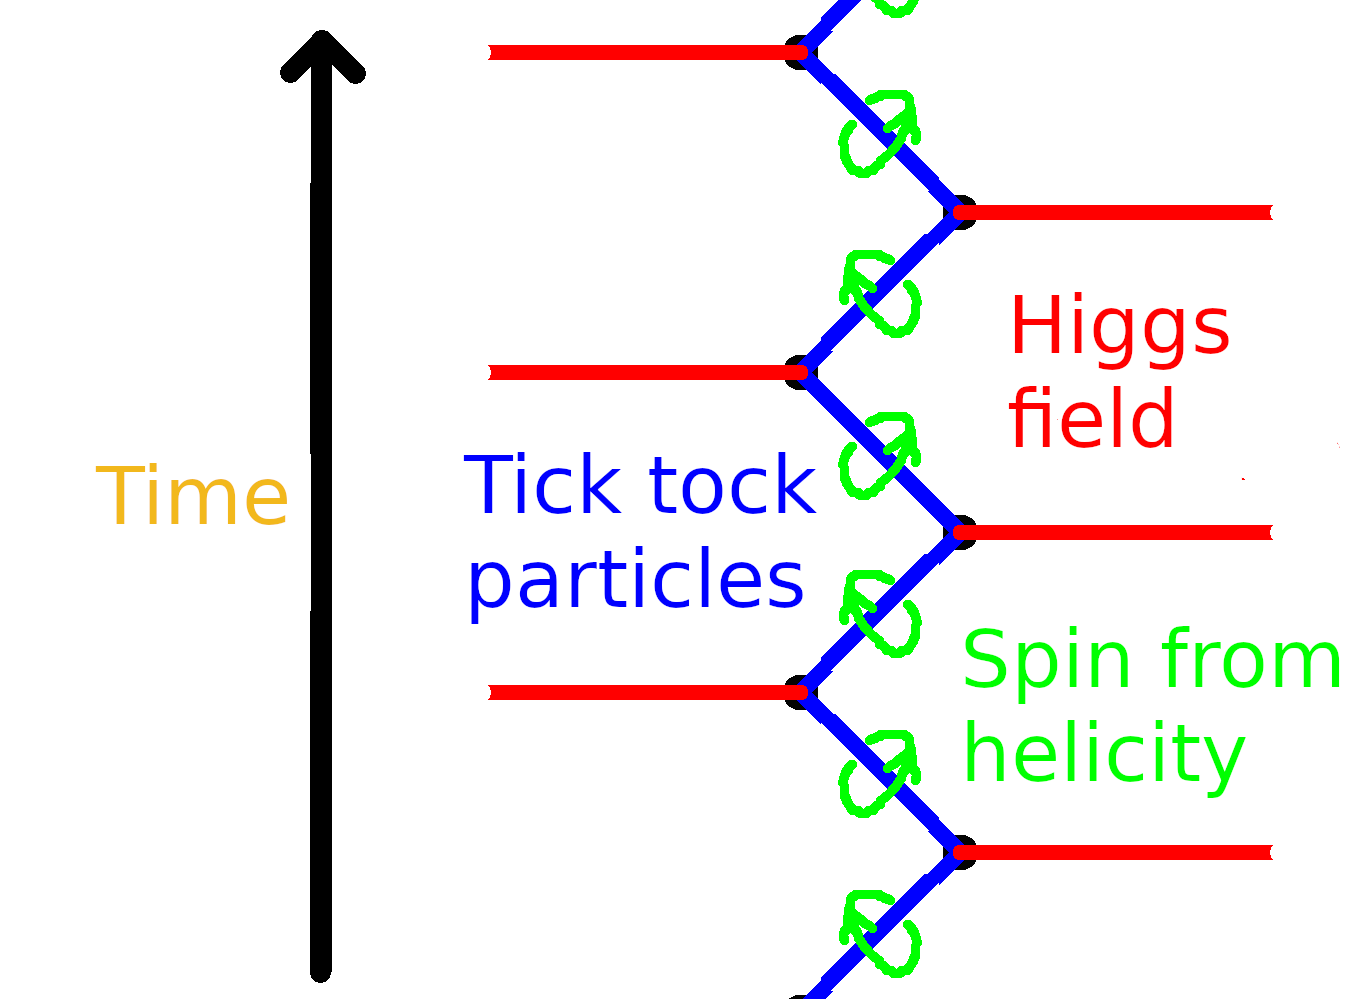
\includegraphics[scale=0.7]{zig_zag_color.png}
\caption{The tick-tock particle picture of the Dirac 
equation, after Penrose~\cite{penrose2006road}. 
A massive electron (blue) alternates between 
right- and left-helicity massless segments, coupled 
at each vertex by the Higgs field (red). The green 
loops indicate spin emerging from the alternating 
helicity, the two $\mathfrak{su}(2)$ factors of 
$\mathfrak{so}(3,1) \cong \mathfrak{su}(2) \times 
\mathfrak{su}(2)$ made visual. Each vertex is a 
handoff event in the sense of 
Section~\ref{sec:handoff}: one quantum of action 
deposited, one helicity outcome recorded, one 
sample of proper time produced. Adapted from~\cite{penrose2006road}. 
Penrose's interpretation of the Dirac equation and 
the Higgs mechanism for an electron.}
\label{zigzag}
\end{figure}

The structural parallel with the bilocal construction 
and the handoff definition is close at the level of 
the Lie algebra decomposition: the two Weyl 
spinors correspond to the two photons emitted by 
$\mathcal{P}$; the Higgs interaction corresponds to 
the absorption events at $\mathcal{R}$ and 
$\mathcal{L}$; between interactions each spinor is 
massless and moves at $c$, a pure carrier. Each 
Higgs interaction is a handoff event in the sense 
of Section~\ref{sec:handoff}: it deposits one 
quantum of action $\hbar$, produces one sample of 
proper time, records one helicity outcome, and 
increments the matter-memory of the particle by 
one Bremermann sample.


The anticorrelated helicity assignment in both constructions 
has a common algebraic origin in the Lie algebra decomposition 
already noted above. The Bisognano--Wichmann modular 
conjugation $J$ acts on right-wedge photon creation operators 
as
%
\begin{equation}
    J\, a^{R\dagger}_{k,\lambda}\, J^{-1} 
    = a^{L\dagger}_{-k,-\lambda},
\end{equation}
%
flipping helicity and reversing the spacelike separation 
direction $R \leftrightarrow L$. The PCT operator $\Theta$ 
acts on a right-handed Weyl spinor as
%
\begin{equation}
    \Theta\, \psi_R(t,\mathbf{x})\, \Theta^{-1} 
    \propto \psi_L(-t,-\mathbf{x}),
\end{equation}
%
flipping helicity and reversing the timelike separation 
direction $t \to -t$. In both cases the operation is the 
same at the representation-theoretic level: exchange of 
the two $\mathfrak{su}(2)$ factors of 
$\mathfrak{so}(3,1) \cong \mathfrak{su}(2) \times 
\mathfrak{su}(2)$, which is what helicity-flip means 
algebraically. The operators $J$ and $\Theta$ act on 
different Hilbert spaces and are not equal; what they 
share is that they both select the same class of 
invariant configuration, anticorrelated helicities,
because PCT-invariance forces that choice 
independently of whether the separation between the two 
helicity sectors is spacelike (Rindler horizon) or 
timelike (Compton worldline). The bilocal Bell state 
and the Dirac 4-spinor are therefore the same 
PCT-invariant structure at different codimension, and 
the Lie algebra is the common home of both.


In this analogy, mass is associated with the 
regularity of these interactions: heuristically, 
a particle is massive because it undergoes repeated 
Higgs interactions at the Compton frequency, and 
its mass is related to that rate via 
$m = h\dot{N}_{Higgs}/c^2$. This is a 
reinterpretation of the standard Higgs mechanism 
in handoff-event language, not a new claim about it.
This is the handoff-event 
reading of $E = \hbar\omega$: mass is not a static 
property but a rate, the frequency at which the 
particle exchanges one quantum of action with the 
Higgs field.
Proper time along a worldline 
is then a foliation by discrete handoff events, 
each separating the causal past from the causal 
future of that interaction, the one-dimensional 
analogue of the Rindler horizon, and
matching the holographic screen picture of 
Verlinde~\cite{entropic}.
This suggests that the one-dimensional handoff 
of the zig-zag and the horizon handoff of the 
bilocal construction are analogous elementary 
events, the timelike and spacelike faces of the 
same PCT-invariant structure.

\subsection{Relation to Existing Programs}
\label{sec:literature}

The matter-substrate framework of this section makes contact 
with two independent programs in quantum foundations that 
approach emergent time from complementary directions.

The Page--Wootters mechanism~\cite{page1983evolution, 
giovannetti2015quantum} derives time evolution relationally: 
a global static state $|\Psi\rangle \in 
\mathcal{H}_{\mathrm{clock}} \otimes \mathcal{H}_{\mathrm{sys}}$ 
satisfying a Wheeler--DeWitt-like constraint yields emergent 
dynamics when conditioned on clock eigenstates $|t\rangle$. 
The mechanism is exact but leaves the physical identity of 
the clock system unspecified. The present framework 
supplies that identity: the matter substrate is the clock, 
with phase $e^{iS/\hbar}$ advancing at the Bremermann rate 
$mc^2/h$. The standard mechanism assumes a continuous clock 
time $t$; the present construction replaces this with a 
discrete sequence of handoff events, each acting as a PVM 
conditioning step that advances the Bremermann count by one 
quantum of action. Proper time is relational in exactly the 
Page--Wootters sense, but the clock states are physical 
rather than abstract.

The modular flow perspective of Connes and 
Rovelli~\cite{connes1994neumann} approaches the same 
problem algebraically. In a generally covariant quantum 
theory the Hamiltonian vanishes on physical states and no 
preferred time exists; Connes and Rovelli show that a state 
$\omega$ on a von Neumann algebra $\mathcal{M}$ nonetheless 
generates a canonical one-parameter automorphism group, the 
modular flow $\sigma_t^\omega$, via Tomita--Takesaki theory. 
This flow satisfies the KMS condition and is 
thermodynamically indistinguishable from thermal time 
evolution. The Bisognano--Wichmann 
theorem~\cite{bisognano1975duality}, already central to 
the PCT structure of Section~\ref{sec:microstates}, 
identifies this modular flow concretely with Rindler time 
evolution for the vacuum restricted to one wedge. The 
connection to the present framework is therefore already 
implicit in the construction: the horizon $\mathcal{H}$ is 
precisely the algebraic cutoff that Connes and Rovelli 
require, restricting the observable algebra to the right 
wedge and generating the modular flow as a consequence. 
What the present framework adds is a discrete substrate 
beneath that flow: the continuous modular parameter is the 
thermodynamic limit of discrete Bremermann samples, and the 
KMS thermal character of the modular flow is the 
ensemble-level expression of the saturation condition of 
Section~\ref{sec:saturation}.

The two programs are thus not independent supports for 
emergent time but complementary descriptions of the same 
structure at different levels: Page--Wootters gives the 
kinematic conditioning on individual clock states, 
Connes--Rovelli gives the thermodynamic flow that emerges 
when those states are coarse-grained across a horizon. The 
matter substrate and the handoff event are the microscopic 
objects that both programs require but neither specifies.

Verlinde's entropic gravity~\cite{entropic} operates at the 
thermodynamic level of the same horizon structure; the 
present framework supplies the microstate layer beneath it, 
with each handoff event realising one entropy increment of 
the kind Verlinde's screens accumulate in bulk. The 
Wigner's friend problem~\cite{brukner2018no} and the 
Frauchiger--Renner theorem~\cite{frauchiger2018quantum} 
identify the multi-observer problem as formally sharp; the 
vocabulary introduced here --- spatial bits, PVM 
projections, handoff events, matter-memory --- is the 
natural language in which that problem must be posed when 
the observers are causally separated by a horizon, a point 
developed in Section~\ref{sec:erepr}.

% Section 5
\section{pp-Wave Geometry and Action}
\label{sec:ppwave}
WLOG we introduce coordinates for the photon traveling from $\mathcal{P}$ $(-1,0)$ to $\mathcal{R}$ $(0,1)$.
We work in the null coordinates $u, v$ defined 
in Section~\ref{sec:microstates}, where the photon propagates along the null plane $u = 0$, $z$ is the longitudinal direction, and $(x,y)$ are transverse coordinates. Then $(u,v)$ = $(0,0)$ is $\mathcal{P}$'s location, $(u,v)$ = $(0,2)$ is $\mathcal{R}$'s location, and $(u,v)$ = $(0,1)$ is the intersection of the photon with the past right Rinder horizon. The situation is reversed for the left moving photon; we swap $u$ and $v$ to describe photon moving from $\mathcal{P}$ to $\mathcal{L}$.

\subsection{The Planar Impulsive Wave: Delocalized Limit}
\label{sec:planar_wave}

When the photon carries zero transverse momentum its energy is uniform 
across the horizon cross-section. The stress tensor at the horizon is
\begin{equation}
    T_{uu}(u,\mathbf{x}_\perp) = \frac{\hbar\omega}{A_\perp}\,\delta(u),
    \label{eq:Tuu_planar}
\end{equation}
where $A_\perp$ is the transverse horizon area and $\delta(u)$ encodes the 
impulsive character of the interaction. The corresponding gravitational 
perturbation is a planar impulsive wave in Brinkmann form
\begin{equation}
    ds^2 = -2\,du\,dv + H_{ij}(u)\,x^i x^j\,du^2 + d\mathbf{x}_\perp^2,
\end{equation}
where the Einstein equation $R_{uu} = 8\pi G T_{uu}$ with 
$R_{uu} = -\tfrac{1}{2}\mathrm{tr}(H_{ij})$ gives
\begin{equation}
    H_{ij}(u) = -\frac{8\pi G\hbar\omega}{A_\perp}\,\delta(u)\,\delta_{ij}.
    \label{eq:H_planar}
\end{equation}

\paragraph{Area increment.}
The Raychaudhuri equation on the null congruence gives
\begin{equation}
    \frac{d\theta}{du} = -8\pi G\,T_{uu} 
    = -\frac{8\pi G\hbar\omega}{A_\perp}\,\delta(u),
\end{equation}
so the expansion receives an impulsive kick 
$\Delta\theta = -8\pi G\hbar\omega/A_\perp$ at $u=0$. 
Integrating over the horizon area:
\begin{equation}
    \boxed{\Delta A = A_\perp\,|\Delta\theta| = 8\pi G\hbar\omega,}
    \label{eq:deltaA_planar}
\end{equation}
identical to the AS result derived in Section~\ref{sec:deltaA}, 
here distributed uniformly rather than concentrated near the beam axis.

\paragraph{Longitudinal shift and BMS structure.}
The gravitational memory of the planar wave is
\begin{equation}
    \Delta v(\mathbf{x}_\perp) 
    = \tfrac{1}{2}\bar{H}_{ij}\,x^i x^j 
    = -\frac{4\pi G\hbar\omega}{A_\perp}\,r^2,
    \label{eq:shift_planar}
\end{equation}
where $\bar{H}_{ij} = \int H_{ij}\,du$. This quadratic shift satisfies 
$\nabla^2_\perp(\Delta v) = -8\pi G\hbar\omega/A_\perp = \mathrm{const}$. 
A constant-Laplacian supertranslation field corresponds to a single 
$\ell = 2$, $m = 0$ solid harmonic in the angular mode decomposition: 
exactly one BMS mode is excited. 
Compare the AS shift $\Delta v \propto -\ln r^2$, whose Laplacian is 
$\nabla^2_\perp(\Delta v) \propto \delta^{(2)}(\mathbf{x}_\perp)$; 
a point-source Laplacian couples to all angular harmonics, 
so the AS wave populates the entire BMS spectrum.

\paragraph{Cut-and-paste structure.}
Despite its delocalized transverse profile, the planar impulsive wave 
retains the cut-and-paste structure of the AS pp-wave: the geometry is 
flat for $u < 0$ and $u > 0$, joined at $u = 0$ by the 
identification~\eqref{eq:shift_planar} together with a transverse 
velocity kick $\Delta\dot{x}^i = \bar{H}^i_{\ j} x^j = 
-(8\pi G\hbar\omega/A_\perp)\,x^i$ directed inward. 
The planar wave is therefore the global, uniform-expansion version 
of the same horizon surgery that the AS wave performs locally.

\subsection{The AS pp-Wave and Its Effects}

Test particles at fixed transverse positions $(x,y)$ experience two effects as the shock front crosses $u = 0$:

\begin{enumerate}
    \item \textbf{Longitudinal shift.} The $v$ coordinate is displaced by
    \begin{equation}
    \Delta v \propto -\ln r^2, \qquad r^2 = x^2 + y^2.
    \end{equation}
    This shift is lightlike: no proper time elapses for a particle crossing the shock, but it is displaced along the null direction. Near the axis ($r \to 0$) the shift diverges, encoding the concentration of energy along the photon's trajectory.

    \item \textbf{Transverse focusing.} The gradient of the longitudinal shift produces a transverse velocity
    \begin{equation}
    \Delta \mathbf{v}_\perp \propto \nabla \ln r \propto \frac{1}{r},
    \end{equation}
    directed toward the axis. Test particles are pulled toward the centre of the wave, regardless of their initial transverse separation.
\end{enumerate}

\subsection{The Longitudinal Shift Makes Space}

The longitudinal shift deserves closer attention, because it carries a meaning beyond a mere coordinate displacement. The photon emitted by $\mathcal{P}$ propagates along the null direction; as it crosses the Rindler horizon, the AS shift displaces the future light cone of every test particle it passes. For the photon traveling into the right wedge, the shift pushes the right wedge's geometry in the $+v$ direction; for the entangled partner traveling into the left wedge, the shift pushes the left wedge in the $-v$ direction. The two wedges are displaced \emph{away from each other} along the longitudinal null direction. See Figure \ref{paz_shift}.

\begin{figure}[h]
\centering
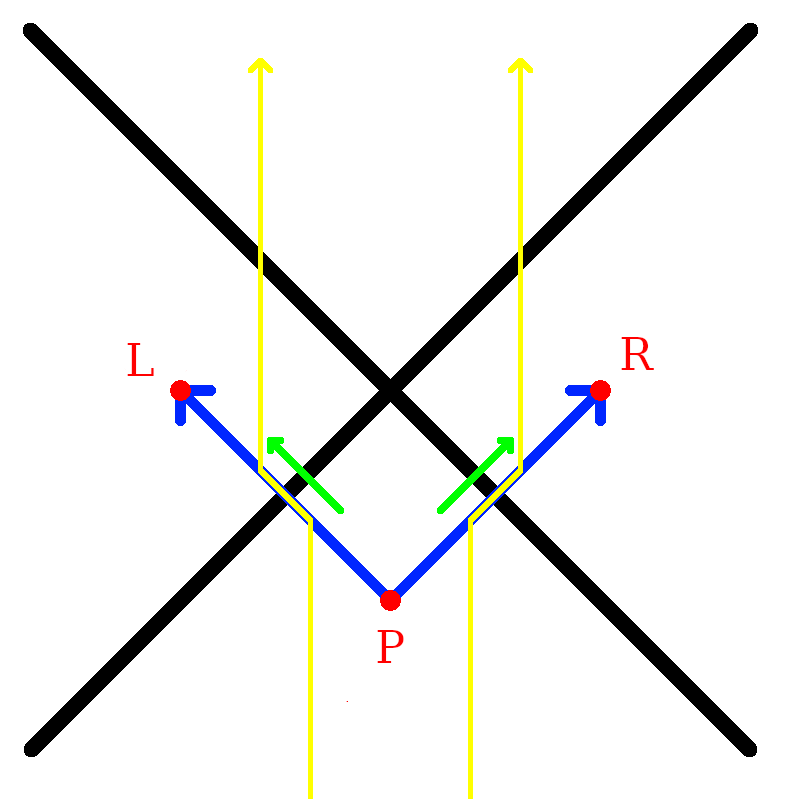
\includegraphics[scale=0.75]{paz_shift.png}
\captionsetup{width=0.7\textwidth}
\caption{The green arrows show the longitudinal shift  that occurs where the photons cross the horizon. Test particles, shown in yellow, are pushed outwards away from $z=0$ due to the creation of space along the null lines originating from $\mathcal{P}$.}
\label{paz_shift}
\end{figure}

At the intersection of the shock front $u=0$ with the past right 
Rindler horizon at $(u,v)=(0,1)$, the transverse $(x,y)$ plane 
is identified with the horizon area elements $dA = dx\,dy$. The 
longitudinal shift $\Delta v \propto -\ln r^2$ displaces the 
horizon outward in the $v$ direction, pushing the right wedge 
geometry away from the horizon. The entangled partner photon 
produces a symmetric shift in the $u$ direction at the left 
Rindler horizon, pushing the left wedge away from its horizon. 
The two wedges are therefore displaced away from their respective 
horizons in opposite null directions.

\subsection{Transverse Focusing Increments Horizon Area}
\label{sec:deltaA}

The Raychaudhuri calculation of Section~\ref{sec:planar_wave} already 
establishes $\Delta A = 8\pi G\hbar\omega$ in the delocalized limit 
via equation~\eqref{eq:deltaA_planar}. We now derive the same result 
for the localized AS pp-wave, confirming that the area increment is 
independent of the transverse localisation of the photon.

The transverse focusing of the AS pp-wave produces a calculable 
increment in horizon area. We derive this using the Raychaudhuri 
equation on the null congruence generating the Rindler horizon, 
following Jacobson~\cite{jacobson1995thermodynamics} and consistent 
with the generalized second law for Rindler horizons proved by 
Wall~\cite{wall2010proof}, but applied here to a single microstate 
rather than a thermodynamic or ensemble average.

For a null congruence with generators $k^\mu$ and expansion 
$\theta$, the Raychaudhuri equation gives
\begin{equation}
\frac{d\theta}{du} = -\tfrac{1}{2}\theta^2 
    - \sigma_{\mu\nu}\sigma^{\mu\nu} 
    - 8\pi G\, T_{\mu\nu} k^\mu k^\nu.
\end{equation}
Integrating over the horizon patch in the linearised regime 
and using $k^\mu = \delta^\mu_u$, the area change is
\begin{equation}
\Delta A = 8\pi G \int T_{uu}\, du\, d^2x_\perp.
\label{eq:deltaA}
\end{equation}
In a strict AS construction, the source is a point particle 
and $T_{\mu\nu}$ is distributional, concentrated on the axis. 
The present construction provides a natural regularization: the 
photon is a normalizable mode of the electromagnetic field in 
double-null gauge, with a smooth transverse profile set by the 
wavelength $\sim c/\omega$. The electromagnetic stress-energy 
$T_{uu}$ is well-defined throughout, integrates to $\hbar\omega$ 
over the transverse plane by energy conservation, and recovers 
the strict AS limit as $\omega \to \infty$ with the logarithmic 
divergence regulated at the scale $c/\omega$.

Substituting into equation~\eqref{eq:deltaA} gives
\begin{equation}
\boxed{\Delta A = 8\pi G\,\hbar\omega = 8\pi G\,\Delta E.}
\label{eq:deltaA_result}
\end{equation}
The horizon area grows by one discrete, calculable increment 
per photon absorbed, microstate by microstate, without 
reference to bulk thermodynamic averages. This is property~(iv) 
of the handoff definition of Section~\ref{sec:handoff} 
verified geometrically: the area increment $\Delta A = 
8\pi G\hbar\omega$ is the geometric expression of one 
quantum of action $\hbar$ deposited into matter-memory 
by one measurement event, with the Planck area $\ell_P^2$ 
as the conversion factor between the two descriptions.

Here the null generators of the horizon are taken to be 
affinely parametrised as $k^\mu = (\partial/\partial u)^\mu$ 
in double-null coordinates, so that $\int T_{uu}\,du\,d^2x_\perp 
= \hbar\omega$ is the total null energy of the photon. This 
differs from the Killing-normalised convention by a factor of 
the surface gravity $\kappa = a$; the two are related by 
$(\partial/\partial u)^\mu = a(\partial/\partial\eta)^\mu$ 
at the horizon, consistent with the standard 
result $\Delta A = 8\pi G E/\kappa$ when $E = \hbar\omega$ 
is the Killing energy.

The longitudinal shift $\Delta v \propto -\ln r^2$ produced by each 
AS pp-wave at the Rindler horizon is a supertranslation in the sense of 
Bondi--Metzner--Sachs (BMS) symmetry. Hawking, Perry, and 
Strominger~\cite{hawking2016soft} showed explicitly that a black 
hole is supertranslated by the passage of an asymmetric shockwave, 
and the AS longitudinal shift is precisely the linearised 
supertranslation field on the horizon. Carlip~\cite{carlip2018black} 
demonstrated that the near-horizon diffeomorphisms of a generic 
black hole are enhanced to a $\mathrm{BMS}_3$ algebra whose central 
charge determines the Bekenstein--Hawking entropy, but his program 
identifies the symmetry without specifying the physical process that 
excites individual modes. The bilocal construction supplies that 
process. The shockwave S-matrix program of 't~Hooft~\cite{hooft1996scattering} 
established that the longitudinal AS shift is the fundamental dynamical 
ingredient for horizon information exchange, working at the level of the
full S-matrix; the present construction realises the same shift at the 
level of a single microstate.
Each measurement event produces one AS pp-wave, which 
deposits one supertranslation at the Rindler horizon, exciting one 
mode of the $\mathrm{BMS}_3$ algebra.
This microstate structure is consistent with Carlip's result: 
the microstates being counted are the measurement events themselves.

This places the bilocal construction inside the 
soft-theorem / gravitational-memory / BMS triangle 
established by Strominger and 
Zhiboedov~\cite{strominger2016gravitational}. Each 
measurement event sits at the intersection of three 
equivalent descriptions: a gravitational memory burst 
(the AS longitudinal shift $\Delta v \propto -\ln r^2$), 
a zero-energy soft graviton insertion (a pole in the 
Weinberg soft graviton 
theorem~\cite{weinberg1965infrared}), and a BMS 
supertranslation mode on the horizon. The bilocal source 
makes this triangle constructive rather than merely 
structural: one emitted photon pair produces one AS 
pp-wave, one supertranslation, and one excited mode of 
the $\mathrm{BMS}_3$ algebra, in a one-to-one 
correspondence. The counting of horizon entropy via the 
$\mathrm{BMS}_3$ central charge~\cite{carlip2018black} 
then acquires a direct operational reading: it counts 
measurement events, one supertranslation mode per 
absorbed photon.

\subsection{The Localization Transition}
\label{sec:loc_transition}

The planar impulsive wave and the AS pp-wave are the two extremes of a 
one-parameter family parametrised by the transverse width $\sigma$ of 
the photon mode. Replacing the uniform density $\hbar\omega/A_\perp$ 
in~\eqref{eq:Tuu_planar} with a normalized Gaussian 
$g_\sigma(\mathbf{x}_\perp) = (\pi\sigma^2)^{-1}e^{-r^2/\sigma^2}$,
\begin{equation}
    T_{uu}(u,\mathbf{x}_\perp) 
    = \hbar\omega\,g_\sigma(\mathbf{x}_\perp)\,\delta(u),
\end{equation}
gives a family that connects the two limits: as $\sigma \to \infty$ 
(at fixed horizon area $A_\perp$) the energy density becomes approximately 
uniform and the shift approaches the quadratic 
form~\eqref{eq:shift_planar}; as $\sigma \to 0$ the energy concentrates 
on the axis and the shift approaches the AS logarithmic 
form~\eqref{eq:shift_AS}. The total null energy $\hbar\omega$ is 
preserved throughout, so
\begin{equation}
    \Delta A = 8\pi G\int T_{uu}\,du\,d^2x_\perp = 8\pi G\hbar\omega
\end{equation}
holds for all $\sigma$. The regulated longitudinal shift of 
Appendix~\ref{sec:as_reg} describes this interpolation in the 
neighbourhood of the AS limit; the natural transverse scale 
is the photon wavelength $\sigma \sim c/\omega$, consistent with 
the regularization scheme of that appendix.

The BMS mode content transitions continuously with $\sigma$. At large 
$\sigma$ the Laplacian $\nabla^2_\perp(\Delta v)$ is approximately 
constant, selecting the $\ell = 2$, $m=0$ mode; as $\sigma$ decreases, 
the Laplacian sharpens toward a delta function and progressively higher 
multipoles are populated until the full BMS spectrum is excited in the 
AS limit.

The localization transition is therefore 
simultaneously a transition in the BMS mode 
content of the horizon perturbation, a 
transition in the spatial distribution of 
the area increment, and the geometric 
counterpart of the POVM-to-PVM transition 
of Section~\ref{sec:pvm_localization}: the 
one-parameter Kraus family~\eqref{eq:kraus_longitudinal} 
parametrized by $\sigma$ has a direct 
geometric image in the interpolation between 
the planar impulsive wave and the AS pp-wave, 
with the Stokes line of~\cite{player2025driving} 
marking the boundary between the two regimes.

\subsection{Action and the Gravitational Boundary}
\label{sec:microstate_action}

The equality derived below is an internal consistency 
check on the microstate identification, not a novel 
result claimed in isolation. The thermodynamic 
interpretation of the GHY boundary term on null 
surfaces is established by Chakraborty and 
Padmanabhan~\cite{chakraborty2020boundary}; the 
broader program of 
Padmanabhan~\cite{padmanabhan2010thermodynamical} 
identifies gravitational boundary terms as the 
fundamental degrees of freedom at the ensemble level. 
What the present construction contributes is not the 
identity $S_{GHY}|_{\mathcal{H}} = S_{\mathrm{matter}}$ 
but its realisation microstate by microstate: if 
individual quantum measurement events genuinely are 
the microstates underlying each area increment, the 
geometric count and the informational count must agree 
event by event. The calculation below verifies that 
they do, closing the consistency loop.


Each absorption event transfers null energy $\hbar\omega_i$ across 
the horizon. The matter action at the horizon is defined as the 
null-surface integral of the stress-energy, evaluated over the 
horizon generators:
%
\begin{equation}
S_{\text{matter}} 
\;=\; \sum_i \int T_{uu}^{(i)}\,du\,d^2x_\perp 
\;=\; \sum_i \hbar\omega_i,
\end{equation}
%
where the second equality follows from energy conservation 
applied to each photon. This is the null-surface analog of 
the worldline action $\int E\,d\tau$: on a null surface the 
affine parameter $u$ plays the role that proper time plays 
on a timelike worldline, and the integral $\int T_{uu}\,du$ 
plays the role of $\int E\,d\tau$. 

The two are not the same integral. After the absorption event, 
the detector's worldline action continues to accumulate as 
$\hbar\omega_i\,\Delta\tau$ for all subsequent proper time 
$\Delta\tau$, encoding the Bremermann memory of the event. 
The equality $S_{GHY}|_{\mathcal{H}} = S_{\text{matter}}$ 
holds for the null-surface version of the matter action, 
evaluated at the moment of horizon crossing; it is a statement 
about the handoff event itself, not about the subsequent 
worldline evolution. The Rindler proper time $\eta$ and the 
affine null parameter $u$ are related by $u \propto e^{-a\eta}$, 
and it is this exponential relation, not a simple 
proportionality, that is responsible for the Unruh 
temperature and that distinguishes the null-surface action 
from the worldline action. This is the 
matter action counted sample by sample: one quantum of action 
per event, one event per emitted pair.

The same events have a geometric description. By 
eq.~\eqref{eq:deltaA_result}, each absorption sample contributes 
a horizon area increment $\Delta A_i = 8\pi G\hbar\omega_i$, so 
the total area increment summed over all events is
%
\begin{equation}
\sum_i \Delta A_i = 8\pi G \sum_i \hbar\omega_i = 8\pi G\, 
S_{\text{matter}}.
\end{equation}
%
This geometric sum has a precise identification in the 
gravitational action. On a stationary Rindler horizon the 
unperturbed expansion of the null generators vanishes, $\theta = 
0$, so the Gibbons--Hawking--York boundary 
term~\cite{gibbons1977action} is sourced entirely by the AS 
pp-wave perturbations:
%
\begin{equation}
S_{GHY}\big|_{\mathcal{H}} 
= \frac{c^4}{8\pi G}\int_{\mathcal{H}} \theta\, d^2x_\perp\, du 
= \frac{c^4}{8\pi G}\sum_i \Delta A_i 
= \frac{c^4}{8\pi G} \cdot 8\pi G\sum_i \hbar\omega_i 
= \sum_i \hbar\omega_i
= S_{\text{matter}}.
\label{eq:GHY_micro}
\end{equation}

Chakraborty and Padmanabhan~\cite{chakraborty2020boundary} showed 
that the gravitational boundary term on null surfaces has a 
thermodynamic interpretation as a heat density $Ts$ of the null 
surface, establishing $S_{GHY}|_{\mathcal{H}} = \text{heat content}$ 
at the level of thermodynamic averages. The present result realises 
the same identity at the level of individual microstates, with each 
contribution to $S_{GHY}$ sourced by a specific quantum measurement 
event rather than a bulk thermal average.

The matter action and the gravitational boundary action are 
therefore equal, event by event, on the stationary Rindler 
horizon. This is not a bulk result: the bulk Einstein--Hilbert 
action vanishes on-shell, and it is the boundary term that 
carries the physical content. The microstate construction 
identifies what that boundary content is: each contribution to 
$S_{GHY}$ corresponds to one quantum of action deposited into 
matter-memory by one measurement event, precisely the handoff 
event of Section~\ref{sec:handoff}. The event-by-event equality 
$S_{GHY}|_{\mathcal{H}} = S_{\mathrm{matter}}$ is therefore 
the geometric consistency check on the information-theoretic 
framework of Section~\ref{sec:substrate}: the Raychaudhuri 
equation and the handoff definition count the same events 
in two languages, and they agree.


The equality $S_{GHY}\big|_{\mathcal{H}} = S_{\text{matter}}$ 
suggests a stronger reading, which we flag as speculative 
but worth stating. The bulk Einstein--Hilbert action 
vanishes on-shell, so it is the boundary term alone that 
carries the gravitational degrees of freedom. If the boundary 
term counts matter action quanta event by event, as 
equation~\eqref{eq:GHY_micro} shows, then the geometry at 
the horizon is not an independent quantity that happens to 
equal the matter action: it \emph{is} the matter action, 
expressed in geometric language. The Planck area $\ell_P^2 = 
\hbar G/c^3$ is the conversion factor between the two 
descriptions, relating one quantum of action $\hbar$ to one 
Planck-area patch on the horizon. In this reading the metric 
near the horizon is not a smooth field that matter happens to 
perturb; it is a coarse-grained count of the action quanta 
that have passed through the horizon surface, with the 
Bekenstein--Hawking area law as the statement that these two 
counts agree. We do not claim to establish this here; it is 
a direction the present construction motivates and that we 
leave for future work. Whether this identification extends 
from the boundary into the bulk, that is, whether the Ricci 
scalar $R$ can be understood as an action-quanta density 
with $\ell_P^2$ as the conversion factor, is the central 
open question.

This result is consistent with and extends programs of 
Jacobson~\cite{jacobson1995thermodynamics} and 
Padmanabhan~\cite{padmanabhan2010thermodynamical}, which argue 
that the gravitational boundary term rather than the bulk 
Einstein--Hilbert action is the fundamental gravitational degree 
of freedom. Those programs establish this at the level of 
thermodynamic averages. The present construction realizes the 
same identification at the level of individual microstates, with 
each boundary contribution sourced by a specific quantum 
measurement event rather than a bulk average. The standard 
result emerges from summing over the ensemble; the microstate 
picture supplies what the thermodynamic programs leave open: 
the physical process underlying each boundary contribution.

The equality $S_{GHY}|_{\mathcal{H}} = S_{\mathrm{matter}}$ 
is structurally related to the Ryu--Takayanagi 
formula~\cite{ryu2006holographic}, which identifies the 
entanglement entropy of a boundary region with the area 
of a minimal bulk surface in AdS: $S_{\mathrm{ent}} = 
A / 4G\hbar$. Three differences sharpen the comparison. 
First, the present result holds in flat Minkowski space 
on a Rindler horizon rather than on a minimal surface in 
AdS, and requires no holographic dual. Second, it is an 
equality of actions rather than of entropies, with the 
Planck area $\ell_P^2$ as the conversion factor between 
the two sides rather than as a fixed coefficient. Third, 
it holds event by event rather than as a thermodynamic 
average over a thermal ensemble: the AS pp-wave sourced 
by a single photon produces a single calculable area 
increment, and summing over events recovers the 
thermodynamic result. Whether 
$S_{GHY}|_{\mathcal{H}} = S_{\mathrm{matter}}$ is the 
flat-space Rindler limit of the Ryu--Takayanagi formula, 
or whether the two results are independent derivations of 
the same underlying holographic principle from orthogonal 
directions, is a natural question for future work.

The classical focusing theorem used above to derive 
$\Delta A = 8\pi G\hbar\omega$ has a quantum 
generalisation, the Quantum Null Energy 
Condition (QNEC)~\cite{bousso2016quantum, 
ceyhan2020recovering}, which replaces the null 
energy condition with a bound involving the second 
derivative of von Neumann entropy of the outgoing 
field state along the null generators. The QNEC is 
the natural framework for extending the present 
construction beyond pure microstates: the classical 
focusing theorem suffices here because the bilocal 
construction maintains a globally pure state 
throughout, with no need to trace out either wedge. 
At the boundary of EFT validity, where the 
single-wedge Rindler description requires tracing 
out $\mathcal{L}$ and the global pure state gives 
way to a mixed thermal state, the QNEC becomes the 
operative inequality; that it saturates precisely 
at $\omega = \omega_{\mathrm{sat}}$ is consistent 
with the six equivalent conditions of 
Proposition~\ref{prop:eft}, and we leave its 
precise role at that boundary for future work.

% Section 6
\section{Entanglement as Spatial Information}
\label{sec:erepr}

The two geometric regimes of Section~\ref{sec:ppwave} carry complementary 
entanglement interpretations. In the delocalized limit, the planar impulsive 
wave uniformly displaces the entire horizon outward in the $+v$ direction 
(right wedge) and $-v$ direction (left wedge): the two wedges are pushed apart 
globally, and the geometric connection between them is generated by the 
entanglement of the full thermofield double state~\eqref{eq:vacuum_vec}. 
This is the ensemble-level version of Van Raamsdonk's 
argument~\cite{van2010building}: the single BMS mode excited by the 
delocalized photon corresponds to a global deformation of the geometry 
connecting the two wedges. In the localized limit, the AS longitudinal 
shift is concentrated in a cylindrical neighbourhood of the photon trajectory: 
the two wedges are displaced apart locally, microstate by microstate, and the 
geometric connection is built up event by event from individual measurement 
interactions. The full Van Raamsdonk picture is the sum of these local events 
over the ensemble; the bilocal construction makes each contributing event explicit.

Van~Raamsdonk~\cite{van2010building} showed, in 
the AdS/CFT setting, that the entanglement entropy between 
two halves of a thermofield double state controls the 
geometry connecting them: reducing entanglement elongates 
the ER bridge until the geometry disconnects entirely. 
The vacuum decomposition~\eqref{eq:vacuum_vec} is 
precisely the thermofield double state~\cite{maldacena2003eternal}, 
now in flat Minkowski space with helicity labels carried 
through. The AS longitudinal shifts of 
Section~\ref{sec:ppwave} are its event-by-event geometric 
output: each measurement event displaces the two wedges 
apart in opposite null directions, creating new coordinate 
space between them.

A potential sign puzzle deserves immediate attention. 
Van~Raamsdonk's argument implies that a maximally 
entangled state (such as the Bell state~\eqref{eq:microstate_vec}) 
should produce maximal geometric \emph{connection} between 
the two sides, whereas the AS shifts push the wedges 
\emph{apart}. The resolution is that outward displacement 
in the present construction is not disconnection but 
creation of interior volume: the two wedges are not 
separating topologically but making room for the geometry 
between them, consistent with the positive longitudinal 
shift generating new Minkowski space rather than a change 
in causal structure. This is the event-by-event 
realisation of Van~Raamsdonk's entanglement-generated 
geometry. Three features go beyond his 
argument: the setting is flat space without an AdS/CFT 
dual; the result holds microstate by microstate rather 
than at the level of entanglement entropy; and the source 
$\mathcal{P}$ is explicit, providing the physical 
mechanism that generates the entanglement.

The bilocal source prepares an anticorrelated Bell 
state~\eqref{eq:microstate_vec}. We consider the simplest 
case: both $\mathcal{R}$ and $\mathcal{L}$ measure in the 
same basis and both obtain a definite outcome, which we 
label $H_+$ or $H_-$. In this case their outcomes are 
perfectly anticorrelated by the Bell state structure, 
independently of which basis is chosen. The question

\begin{center}
\textit{``who observed $H_+$?''}
\end{center}
then has a binary answer: 
$\mathcal{L}$ (left wedge) or $\mathcal{R}$ (right wedge). 
This is a \emph{spatial bit}, a bit that encodes not a 
polarization state but a location in space. The spatial bit is where the observer-relativity of 
the construction becomes acute. From $\mathcal{R}$'s 
perspective the answer to \textit{``who observed 
$H_+$?''} is a definite classical fact, recorded in 
matter-memory. From $\mathcal{P}$'s perspective before 
any measurement, the answer is indeterminate: the Bell 
state assigns no definite location to $H_+$. From the 
full Minkowski perspective after both measurements, the 
two records are perfectly correlated but the question 
of \emph{when} the spatial fact became definite has no 
observer-independent answer. A PVM by $\mathcal{R}$ on 
a Bell state does not reveal a pre-existing spatial 
fact; it \emph{creates} the spatial bit as a classical 
record in $\mathcal{R}$'s matter-memory.
This is the same PVM projection as 
Section~\ref{sec:pvm_localization}, now read 
informationally rather than geometrically: 
the projection that selects the localized 
microstate from the thermofield double is 
the same event as the projection that creates 
the spatial bit in matter-memory.

Whether that creation is an objective event or a 
relational one is a question the present construction 
does not need to resolve in full generality. Within 
this construction, the spatial bit is relational but 
not arbitrary: its creation is grounded in the common 
causal ancestry of $\mathcal{P}$, which enforces the 
anticorrelation between $\mathcal{R}$'s and 
$\mathcal{L}$'s records as a consequence of shared 
causal history rather than an objective collapse.

Each measurement event has exactly two
irreducible constituents: one quantum of action $\hbar$ written persistently into the
detector's matter-memory as a series of samples, and one bit of polarization registered as a classical
outcome. The entanglement between $\mathcal{R}$ and $\mathcal{L}$ is consumed in producing these two
records, an increase in sampling rate and one bit at each wedge.
What remains after measurement is not the entanglement itself 
but its classical residue: the perfect anticorrelation between
the two bits, and the correlated pair of samples written into the matter on each side of the
horizon. The spatial bit is precisely the polarization bit 
now read as a location rather than a spin state: the same bit that records \emph{what} was
observed also records \emph{where}, because in this construction the two wedges carry
opposite helicities by design. This double duty is forced: the 
anticorrelated helicity assignment of the bilocal source makes 
the two wedges distinguishable by construction, so the spatial 
bit is already latent in the source geometry before any 
measurement occurs.

The information is carried by the matter of the detectors, not by the horizon. As
established in Section~\ref{sec:substrate}, the horizon is a boundary that makes the
left/right distinction sharp; it is the matter on each side that accumulates the samples and
holds the classical record. $\mathcal{R}$'s detector has absorbed one photon, increased its sampling rate, and registered polarization $H_+/H_-$. $\mathcal{L}$'s detector has absorbed one photon, increased its sampling rate, and registered polarization $H_-/H_+$. The two records are perfectly complementary by the anticorrelated structure of the bilocal source, and their complementarity is encoded in matter and is reflected in geometry.

\subsection{Emergent Space and the Thermofield Double}
The Unruh vacuum is the thermofield double state of the left 
and right Rindler wedges~\cite{maldacena2013cool}: 
equation~\eqref{eq:vacuum_vec} is precisely this state, with 
the helicity label $\lambda$ carried through. The bilocal 
source selects one term from this sum at fixed $\omega$ and 
fixed helicity pair, yielding the single 
microstate~\eqref{eq:microstate_vec}. The correlated AS 
longitudinal shifts in opposite null directions are the 
geometric output of this microstate: a linearized perturbation 
of flat Minkowski space that displaces the two wedges away from 
their respective horizons, creating new coordinate space between 
them.

The connection between the two wedges requires no exotic 
geometry: $\mathcal{R}$ and $\mathcal{L}$ are correlated 
because they share a common causal past in $\mathcal{P}$, 
which is ordinary retarded causality. Non-traversability is 
equally automatic,  no signal can pass directly from 
$\mathcal{L}$ to $\mathcal{R}$ because the causal structure 
of Minkowski space forbids it, matching the no-communication 
theorem on the EPR side without additional assumptions. The 
ER=EPR correspondence, in this flat-space setting, reduces to 
the statement that entangled systems with a common causal 
ancestor generate correlated geometric displacements,  a 
consequence of energy--momentum conservation at $\mathcal{P}$ 
rather than a postulate about wormhole topology. The wormhole 
picture of ER=EPR may be what this flat-space causal structure 
looks like in AdS, when the source $\mathcal{P}$ is not 
explicitly available and the connection between wedges must be 
encoded in the geometry itself.

\subsection{Observer-Relativity and the Multi-Observer Problem}
The construction is naturally multi-observer rather than 
single-frame. Standard QFT in the S-matrix formulation 
assumes a single asymptotic observer who prepares the 
initial state and measures the final state; in the 
language of Section~\ref{sec:types}, there is one lab 
and one measurement at the end. Horizon physics 
requires a different framework: four observers 
$\mathcal{P}$, $\mathcal{R}$, $\mathcal{L}$, 
$\mathcal{F}$ each hold partial, causally 
complementary information about the same physical 
process. Neither $\mathcal{R}$ nor $\mathcal{L}$ alone 
can reconstruct the emission at $\mathcal{P}$; their 
two classical bits together can. The horizon is not 
a barrier in a single-observer description but a 
surface that makes the multi-observer structure of 
the construction sharp: it is the boundary at which 
$\mathcal{R}$'s and $\mathcal{L}$'s causal domains 
separate. This is not a limitation of the framework 
but its natural setting, and it is structurally the 
same situation that arises in Wigner's friend 
scenarios~\cite{brukner2018no} applied to 
gravitational systems, a point developed in the following section.

The multi-observer structure exposed here is not 
merely an analogy with Wigner's friend: it is 
precisely that scenario, instantiated in a 
gravitational context with causal separation enforced 
by a horizon rather than by a laboratory door.

A complete formalism for multi-observer quantum 
mechanics, one that specifies consistently how 
causally separated observers' measurement records 
combine into a single description, does not yet 
exist. The Wigner's friend no-go 
theorems~\cite{brukner2018no} and the 
Frauchiger--Renner result~\cite{frauchiger2018quantum} 
establish that the problem is sharp; the relational, 
QBist, and Everettian programs each dissolve it 
differently rather than solving it. The present 
construction operates within a single observer's 
description but does not treat the gap as a 
liability: the observer-independence of the 
Bekenstein--Hawking area law emerges here not from 
a completed multi-observer formalism but from the 
common causal ancestry of $\mathcal{P}$, which 
enforces intersubjective consistency between 
$\mathcal{R}$'s and $\mathcal{L}$'s records without 
requiring an objective wavefunction. The 
Frauchiger--Renner and Wigner's friend problems 
remain open in general; the construction shows that 
causal ancestry is sufficient to ground 
intersubjective agreement in this specific setting.

Whether the relational~\cite{rovelli1996relational}, 
QBist~\cite{fuchs2014introducing}, or Everettian 
frameworks are inequivalent in this setting is an 
open question with physical consequences:
different resolutions imply different answers to whether 
$\mathcal{R}$'s microstate count and $\mathcal{L}$'s 
microstate count are consistent as objective facts 
or only as relational ones. The information-theoretic 
objects introduced here, the spatial bit, the PVM 
projection, the handoff event, the matter-memory, are 
the vocabulary in which that question must eventually 
be posed, but they do not answer it. Multi-observer 
quantum mechanics in the presence of horizons is 
largely uncharted, and the present construction 
should be read partly as a map of that problem space.

% Section 7
\section{Carnot Cycle from Unruh--Landauer}
\label{sec:carnot}

The Carnot cycle developed here is evaluated at the saturation 
frequency $\omega_{\mathrm{sat}} = a\ln 2/c$ of 
Section~\ref{sec:saturation}, the unique frequency 
at which a single photon deposits exactly one bit 
of Bremermann channel capacity per Rindler period. 
At this frequency the Unruh temperature 
$k_BT_H = \hbar a/2\pi c$ and the photon energy 
$\hbar\omega_{\mathrm{sat}} = \hbar a\ln 2/c$ are 
related by
%
\begin{equation}
    k_BT_H = \frac{\hbar\omega_{\mathrm{sat}}}{\ln 2},
    \label{eq:TH_sat}
\end{equation}
%
which is $k_BT_H \sim \hbar\omega_{\mathrm{sat}}$ 
up to the factor $1/\ln 2 \approx 1.44$, the 
nats-to-bits conversion. This factor has a precise 
meaning in the present framework: it is the ratio 
between the natural information unit of the Unruh 
thermal distribution (nats, set by $e$) and the 
binary unit of the helicity outcome (bits, set by 
$\ln 2$). Throughout this section we absorb this 
factor into the order-of-magnitude identification
%
\begin{equation}
    k_BT_H \sim \hbar\omega_{\mathrm{sat}},
    \label{eq:TH_order}
\end{equation}
%
consistent with the heuristic character of the 
Schwarzschild radius and surface gravity 
derivations of Section~\ref{sec:heuristics}, 
where numerical prefactors of the same order 
appear for the same reason. The precise 
coefficient is recovered by working in nats 
throughout, in which case $\ln 2 \to 1$ and 
equation~\eqref{eq:TH_sat} becomes exact. The 
six equivalent conditions of the upcoming
Proposition~\ref{prop:eft} all reduce to 
$\omega = \omega_{\mathrm{sat}}$ at the horizon, 
so evaluating the cycle at this frequency is not 
an additional assumption but the condition that 
the EFT, which we will explore in the next section, is at its natural boundary.

The Carnot cycle developed here is formulated at the level of 
individual non-thermal microstates, and this is the point. 
Reversibility is a feature of the microstate description: in a 
coarse-grained thermal treatment individual microstates are 
inaccessible and the cycle could not be run explicitly. Temperature 
appears in this section not as a primitive imported from the Rindler 
description but as a derived label on each leg of the cycle, 
consistent with the non-thermal Minkowski vantage point maintained 
throughout. The Carnot efficiency bound and the Unruh--Landauer 
bound will emerge as the same inequality viewed from opposite sides 
of this microstate-level construction, closing the loop opened in 
Section~\ref{sec:heuristics}.

We consider in this section the case where $\mathcal{L}$ and $\mathcal{R}$ are moving mirrors being accelerated with an outward thrust from our past bilocal source $\mathcal{P}$ emission, see Figure \ref{carnot}. We complete our bilocal microstate absorption example by reflecting and emitting the photons off of the mirrors.


This reflects the energy back to the future sink 
$\mathcal{F}$, located at $(t,z) = (1,0)$, which is 
the PCT image of $\mathcal{P}$ under the combined 
time-reversal and parity operation that swaps past 
and future wedges. $\mathcal{F}$ plays the role of 
a final absorber, receiving the reflected photons 
and resetting the field state; its existence is 
required by the reversibility of the ideal mirror 
cycle and by the PCT symmetry of the bilocal 
construction. The reflection is reversible in the 
sense that the mirrors do not retain a persistent 
copy of the information that they temporarily store.

The mirrors are ideal, in the sense that they do not retain a persistent copy of the information that they temporarily store; they forget and emit. It is this reversibility that allows us to construct a example of a Carnot cycle at the level of microstates. The working system is the photon–mirror interaction degree of freedom; the Rindler wedge defines the thermal reservoirs, and the mirror trajectory defines the work parameter.

\begin{figure}[h]
\centering
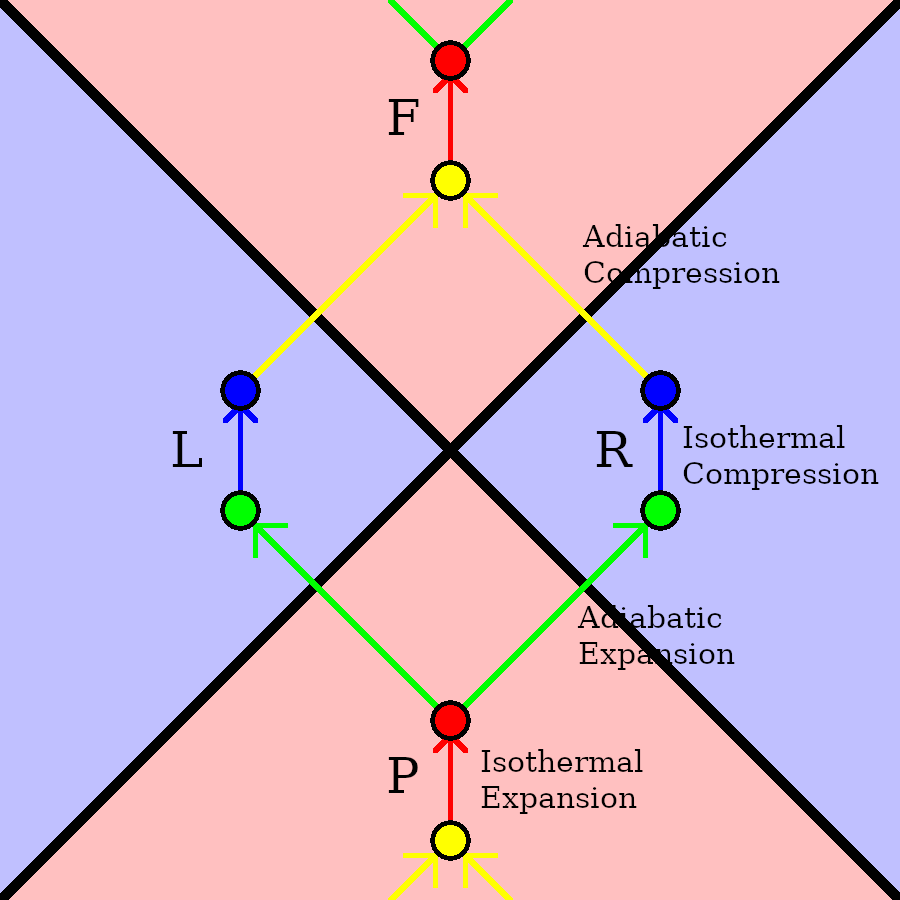
\includegraphics[scale=0.75]{carnot.png}
\captionsetup{width=0.7\textwidth}
\caption{Carnot Cycle: Past ($\mathcal{P}$) bilocal source emits entangled pair with one leg hitting a moving mirror in the right wedge ($\mathcal{R}$). Reflection focuses to a future sink ($\mathcal{F}$). A similar balancing situation exists in the left wedge.}
\label{carnot}
\end{figure}

Consider the point of view of the right Rindler observer $\mathcal{R}$ who sees the event horizon as a thermal object.
The Rindler horizon plays the role of the hot reservoir 
at the Unruh temperature $T_H = \hbar a/2\pi k_B c$, 
consistent with the standard identification of the 
horizon as a thermal object and its connection to the 
generalised second law~\cite{unruh1982acceleration}.
The Rindler wedge interior, where the mirror operates, 
is taken as the cold reservoir at temperature $T_C$. The 
identification of $T_C$ with the Landauer erasure temperature 
of the mirror is an ansatz of the present construction; its 
precise value determines the Carnot efficiency $\eta = 1 - T_C/T_H$.

\begin{itemize} 
\item {\bf Isothermal Expansion:} The bilocal source prepares an entangled photon pair in the basis that $\mathcal{R}$ measures in ($H_+/H_-$ see section \ref{sec:erepr}). In this basis, the Shannon entropy of the Rindler outcome distribution increases from 0 to 1 bit, reflecting the transition from a deterministic prior state to a maximally uncertain Bell state induced by the bilocal entanglement structure,
  , i.e.\ the inverse of the PVM projection 
of Section~\ref{sec:pvm_localization}: 
the isothermal expansion runs the projection 
backward, from a sharp microstate to the 
full superposition; notionally ``drawing some heat from the environment $\mathcal{P}$''.
\item {\bf Adiabatic Expansion:} This corresponds to the crossing over the past Rindler horizon from hot to cold, the absorption of the photon by the mirror.
\item {\bf Isothermal Compression:} This corresponds to controlled 
erasure of the detector's stored bit during the re-emission of the photon 
by the mirror.
This is where the Landauer cost is 
paid~\cite{landauer1961irreversibility, 
bennett1982thermodynamics}: Bennett showed that 
measurement can in principle be performed 
reversibly; it is the erasure of the stored bit 
at re-emission that necessarily dissipates energy, 
at minimum $k_BT_C \ln 2$ into the cold reservoir.
\item {\bf Adiabatic Compression:} This corresponds to the crossing over the future Rindler horizon from cold to hot, the absorption of the future sink $\mathcal{F}$ and reseting of the state to an eigenstate of $H_+$ or $H_-$, zero bits of Shannon entropy. 
\end{itemize}


\subsection{Shannon Entropy, QBism, and 
Wigner's Friend}

The entropy variation in the isothermal legs should be 
understood as Shannon entropy associated with 
measurement outcomes in a fixed operational basis, 
rather than the von Neumann entropy of the global 
quantum state, which remains pure throughout. This 
distinction has a precise foundation. The four-observer 
structure $\mathcal{P}$--$\mathcal{R}$--$\mathcal{L}$--$\mathcal{F}$ 
is a gravitational realisation of the Wigner's friend 
scenario~\cite{brukner2018no}: $\mathcal{P}$ 
prepares the Bell state (Wigner's role), 
$\mathcal{R}$ and $\mathcal{L}$ each measure it 
(the friends' roles), and the question of when 
``collapse'' occurred is observer-relative. From 
$\mathcal{R}$'s perspective, the state collapsed 
upon photon absorption; from the full Minkowski 
perspective, the global state remained pure 
throughout. These descriptions are not contradictory 
but complementary.

The QBist framework~\cite{fuchs2014introducing} resolves 
this cleanly, and is the natural home of the present 
construction. In QBism, quantum states encode an 
agent's beliefs rather than objective microstate 
facts; the correlations between agents' outcomes 
are objectively real and correctly predicted by the 
Bell state structure, but no single agent holds the 
``true'' global state. Each observer's Shannon 
entropy, the uncertainty in their helicity 
outcome prior to measurement, is valid relative 
to them. The Carnot cycle is therefore formulated 
relative to $\mathcal{R}$: its Shannon entropy 
increases from zero to one bit on the isothermal 
expansion leg, decreases on the isothermal 
compression leg, and the area of the cycle in 
$T$-$H$ space is the work extracted, all defined 
by $\mathcal{R}$'s operational measurement basis.

No decoherence assumption is required; Shannon 
entropy here is defined over the classical outcome 
distribution induced by a fixed measurement basis 
(the Rindler detector algebra), independent of the 
unitary evolution of the global state. The objectivity 
of the Bekenstein--Hawking area count is not in 
tension with the observer-relativity of the 
individual microstate: the area increment 
$\Delta A = 8\pi G\hbar\omega$ is a covariant 
physical event, while the assignment of that event 
to a particular observer's measurement record is 
relational. Thermodynamic entropy, in this reading, 
is the classical face of quantum observer-relativity: 
it measures what a given agent does not yet know, 
and its increase under measurement is the same 
process as the Bayesian update arrow of 
Figure~\ref{fig:diagram}, now with a thermodynamic 
label attached.

The interpretational position underlying the 
construction deserves to be stated explicitly. 
Quantum information is treated here as an 
extension of classical information rather than 
a replacement for it. A Hilbert space of 
dimension $2^n$ for $n$ qubits has the same 
dimensional structure as the probability space 
of $n$ classical bits: the statement that two 
coins are correlated as HH or TT but never HT 
or TH already requires a $2^2$-dimensional 
description, and the Bell 
state~\eqref{eq:microstate_vec} is the quantum 
analog of exactly such a classical correlation, 
with probability amplitudes replacing 
probabilities. Quantum observation is 
correspondingly the quantum analog of Bayesian 
conditionalization: the PVM projection updates 
an agent's probability assignment upon receipt 
of a classical outcome. No commitment to a 
specific ontology is required to say this.

The stand the construction takes enters 
precisely at the PVM rule: each handoff event 
is a projective measurement, and its outcome,
the helicity eigenvalue, the spatial bit, 
is recorded in the observer's matter-memory as 
a persistent classical fact. Memory is what 
grounds an observer in their particular 
sequence of outcomes. To interfere with an 
observer who recorded $H_+$ would require 
erasing that record; without erasure, the 
memory distinguishes the two outcomes and no 
interference is possible. The Carnot cycle's 
isothermal compression step is the precise 
physical implementation of this: the mirror 
forgets the bit it learned, paying the Landauer 
cost $k_BT_C\ln 2$. The ideal mirror limit 
$T_C\to 0$ is the limit of perfect forgetting 
at zero thermodynamic cost; the condition 
$T_C>0$ is the condition that some memory 
persists and some coherence is permanently 
lost. The paper does not resolve whether 
perfect forgetting constitutes a transition 
between Everettian branches or a local reset 
of the field state; it shows that the 
thermodynamic cost of forgetting is real and 
precisely calculable, and that the spatial bit, 
the PVM, the matter-memory, and the Landauer 
erasure are the vocabulary in which that 
question must eventually be posed.

\subsection{Work and Efficiency}

The thermodynamic state space of the cycle is parameterised 
by temperature $T$ and Shannon entropy $H$. The two 
isothermal legs operate at $T_H$ and $T_C$ respectively, 
and the entropy change per cycle is exactly one bit:
%
\begin{equation}
\Delta H = \ln 2 \quad \text{(one binary helicity outcome)},
\end{equation}
%
so the work extracted per cycle is the area of the rectangle 
in $T$-$H$ space:
%
\begin{equation}
W = (T_H - T_C)\,\Delta H = (T_H - T_C)\ln 2.
\label{eq:carnot_work}
\end{equation}
%
The work done on the mirror by absorbing one photon of energy 
$\hbar\omega$ is the radiation pressure impulse $\Delta p = 
\hbar\omega/c$, which is responsible for the mirror's 
acceleration into the Rindler wedge. This identifies the hot 
reservoir temperature via
%
\begin{equation}
k_BT_H = \hbar\omega,
\label{eq:TH}
\end{equation}
%
the energy of one photon sets the Unruh temperature of the 
horizon. The Carnot efficiency bound $W \leq T_H\Delta H$ 
then gives
%
\begin{equation}
W \leq \hbar\omega\ln 2 = \frac{\hbar a \ln 2}{2\pi c},
\label{eq:carnot_bound}
\end{equation}
%
where in the last step we used $k_BT_H = \hbar a/2\pi k_Bc$ 
from the Unruh temperature. This is precisely the 
Unruh--Landauer bound~\eqref{eq:UL} at $\Delta H = \ln 2$:
%
\begin{equation}
\boxed{W \leq \frac{\hbar a}{2\pi c}\Delta H 
\iff \Delta E \geq \frac{\hbar a}{2\pi c}\Delta H.}
\label{eq:carnot_UL}
\end{equation}
%
The Carnot efficiency bound for this cycle and the 
Unruh--Landauer bound are therefore the same inequality, 
approached from opposite directions: the Carnot bound is a 
statement about the maximum work extractable from the thermal 
gradient between the horizon and the wedge interior, while 
the Unruh--Landauer bound is a statement about the minimum 
energy cost of acquiring one bit at that horizon. Their 
equivalence identifies the Rindler horizon as a Carnot engine 
operating at the Unruh temperature, with quantum measurement 
as the working substance and the classical bit as the 
thermodynamic output.

The classical precursor to this equivalence is the 
Geroch process~\cite{bekenstein}: a box of radiation 
lowered toward a black hole on a string extracts work 
until, at the horizon, the box carries zero energy 
from the perspective of an observer at infinity. 
Bekenstein showed that dropping the box in must 
increase the black hole's area, establishing a maximum 
efficiency for work extraction that saves the second 
law~\cite{bekenstein}. Our mirror plays the role of 
the box, the measurement impulse plays the role of 
the string tension, and the Unruh--Landauer bound is 
Bekenstein's efficiency constraint expressed in the 
language of information acquisition at the Rindler 
horizon. The two bounds are not merely analogous; 
they are the same inequality, with the Geroch process 
as its classical limit and the Carnot cycle here as 
its microstate realisation.

The cold reservoir temperature $T_C$ is the Landauer 
temperature associated with isolating the mirror from 
its local re-emission environment, while $T_H$ is the 
Landauer temperature associated with isolating the entire 
Rindler wedge from the global Minkowski vacuum. The two 
temperatures correspond to two levels of coarse-graining: 
$T_H$ traces out the opposite wedge at the Rindler horizon, 
while $T_C$ traces out only the mirror's local photon field 
at the scale of the mirror interaction. The temperature 
gradient $T_H > T_C$ is therefore a gradient between 
two scales of isolation, and the Carnot efficiency 
$\eta = 1 - T_C/T_H$ measures how much of the global 
thermal gradient is captured by the local mirror 
interaction. In the limit $T_C \to 0$ the mirror's 
local environment is fully decoupled and the cycle 
extracts maximum work; in the limit $T_C \to T_H$ 
the two scales of isolation coincide and the cycle 
is in hydrostatic equilibrium with no net work extracted.


The efficiency $\eta = 1 - T_C/T_H$ is 
maximised in the limit $T_C \to 0$, which corresponds to 
perfect erasure at zero thermodynamic cost, the ideal 
mirror limit. Any residual $T_C > 0$ reflects irreversibility 
in the mirror's erasure process, consistent with Landauer's 
principle applied to the re-emission step.

% Section 8
\section{Effective Field Theory Structure}
\label{sec:eft}

The bilocal construction has a natural effective 
field theory interpretation. The right wedge 
$\mathcal{R}$ is the \emph{system}, with energy 
scale $E_{\text{sys}}$; the full Minkowski space 
$\mathcal{R} \cup \mathcal{L}$ is the 
\emph{environment}, with energy scale 
$E_{\text{env}} = E_{\text{sys}} + E_\mathcal{L}$. 
The Rindler horizon is the EFT cutoff surface: 
it is the boundary at which the system's 
description and the full Minkowski description 
become incompatible, and the left wedge 
$\mathcal{L}$ is precisely the degrees of freedom 
that the system has integrated out.

\subsection{The GHY Term as Effective Action}
\label{sec:eft_ghy}

We now show that the GHY boundary term arises 
as the effective action for $\mathcal{H}_R$ after 
integrating out $\mathcal{H}_L$ in the path 
integral, elevating the identification 
$S_{GHY}|_\mathcal{H} = S_{\text{matter}}$ from 
Section~\ref{sec:ppwave} from an algebraic 
observation to a structural result.

\paragraph{Setup.}
The full Euclidean path integral for gravity and 
matter decomposes over the two wedges as
%
\begin{equation}
Z = \int \mathcal{D}g_R\,\mathcal{D}\phi_R
    \int \mathcal{D}g_L\,\mathcal{D}\phi_L\;
    e^{-S_R - S_L - S_{\mathcal{H}}},
\end{equation}
%
where $S_{\mathcal{H}}$ is the boundary term at 
the horizon coupling the two wedges. Integrating 
out the left wedge defines the effective action:
%
\begin{equation}
e^{-S_{\text{eff}}[g_R,\phi_R]}
= \int \mathcal{D}g_L\,\mathcal{D}\phi_L\;
  e^{-S_L - S_{\mathcal{H}}}.
\label{eq:eff_action_def}
\end{equation}

\paragraph{Origin of the horizon coupling.}
Integration by parts applied to any kinetic term 
produces a boundary contribution at $\mathcal{H}$. 
For the gravitational field this is the 
Gibbons--Hawking--York term~\cite{gibbons1977action}
%
\begin{equation}
S_{\mathcal{H}} = S_{GHY}\big|_{\mathcal{H}} 
= \frac{1}{8\pi G}\int_{\mathcal{H}} 
  d^2x_\perp\,d\lambda\;\theta,
\end{equation}
%
which couples the two wedge geometries through 
their expansion $\theta$ at the horizon, precisely 
as a scalar kinetic term couples $\phi_L$ and 
$\phi_R$ through their normal derivatives.

\paragraph{Saddle point evaluation.}
The classical solution in the left wedge is flat 
Minkowski space perturbed by the AS pp-wave of the 
left-moving photon. Aichelburg--Sexl pp-waves are 
Ricci flat ($R_{\mu\nu} = 0$) in vacuum, so the 
bulk Einstein--Hilbert action vanishes on-shell:
%
\begin{equation}
S_L\big|_{\text{on-shell}} 
= \frac{1}{16\pi G}\int_L d^4x\sqrt{g}\,R = 0.
\end{equation}

In a standard EFT path integral, integrating out 
the left wedge would produce two contributions: 
the gravitational boundary term $S_{GHY}$ (from 
integration by parts of the bulk kinetic term) 
and the matter action $S_{\text{matter}}^L$ 
(from the left-moving photon). Treated as 
independent, these would give 
$e^{-S_{GHY} - S_{\text{matter}}^L}$, 
and the effective action would be 
$S_R + S_{GHY} + S_{\text{matter}}^L = 
S_R + 2\hbar\omega$.

The consistency check of 
Section~\ref{sec:ppwave} resolves this: 
$S_{GHY}$ and $S_{\text{matter}}^L$ are not 
independent contributions but two descriptions 
of the same physical event, one photon 
crossing the horizon, counted geometrically 
and informationally. Adding them separately 
double-counts that event. The correct horizon 
coupling is therefore $S_{\mathcal{H}} = 
S_{GHY}$ alone, with $S_{\text{matter}}^L$ 
already subsumed into the geometric boundary 
term. At the saddle point:
%
\begin{equation}
\left.
\int \mathcal{D}g_L\,\mathcal{D}\phi_L\;
e^{-S_L - S_{\mathcal{H}}}
\right|_{\text{saddle}}
= e^{-S_{GHY}|_{\mathcal{H}}},
\end{equation}
%
where $S_L|_{\text{on-shell}} = 0$ by 
Ricci-flatness, and the effective action for 
the right wedge is

Since $S_{GHY}|_{\mathcal{H}} = 
S_{\text{matter}}^L = \sum_i\hbar\omega_i$ 
by equation~\eqref{eq:GHY_micro}, the effective 
action for the right wedge is
%
\begin{equation}
\boxed{
S_{\text{eff}}[g_R,\phi_R]
= S_R[g_R,\phi_R] + S_{GHY}\big|_{\mathcal{H}}.
}
\label{eq:Seff}
\end{equation}
%
The GHY term is the contribution to the right 
wedge effective action from integrating out the 
left wedge at the classical level. The bulk left 
wedge action vanishes by Ricci-flatness of the 
AS solution; the entire left wedge effect is 
encoded in the boundary term at the horizon.

\paragraph{Quantum corrections.}
Fluctuations of $\phi_L$ around the saddle 
generate corrections to $S_{\text{eff}}$ 
suppressed by $\ell_P^2/A$ relative to the 
classical term. These are the standard 
entanglement entropy contributions studied by 
Susskind--Uglum~\cite{susskind1994black} and 
Callan--Wilczek~\cite{callan1994geometric}, 
whose UV divergences renormalize Newton's 
constant $G$. Equation~\eqref{eq:Seff} is the 
leading classical contribution.

\subsection{Partition Function and S-Matrix}
\label{sec:eft_partition}

The thermal partition function of the right wedge
%
\begin{equation}
Z = \mathrm{Tr}_{\mathcal{H}_R}\,
    e^{-H_R/k_BT_H}
\end{equation}
%
is obtained from the full Minkowski vacuum by 
tracing out $\mathcal{H}_L$: integrating out the 
left wedge in the path integral yields the thermal 
density matrix for $\mathcal{H}_R$, and $\ln Z$ 
generates the connected correlation functions of 
the right wedge EFT. The S-matrix of the full 
bilocal construction connects the past state at 
$\mathcal{P}$ to the future sink $\mathcal{F}$:
%
\begin{equation}
S = \langle\mathcal{F}|\mathcal{P}\rangle
  = \mathrm{Tr}\,e^{-iHt/\hbar},
\end{equation}
%
which under Wick rotation $\tau = it$ becomes 
$Z = \mathrm{Tr}\,e^{-H\tau/\hbar}$. The Carnot 
cycle of Section~\ref{sec:carnot} is therefore 
the thermodynamic avatar of this S-matrix element: 
the real-time bilocal construction and its 
thermodynamic description are related by Wick 
rotation, and each microstate~\eqref{eq:microstate_vec} 
contributes one term to $Z$ rather than the full 
thermal trace.

\subsection{Horizon Complementarity}
\label{sec:eft_complementarity}

The identification of $\mathcal{H}_R$ as system 
and $\mathcal{H}_L \otimes \mathcal{H}_R$ as 
environment is the operational content of horizon 
complementarity~\cite{susskind1993stretched}: the 
right wedge observer sees a thermal state at $T_H$, 
while the full Minkowski observer sees a pure 
entangled state. These are the EFT and UV 
descriptions of the same microstate. The spatial 
bit, the answer to ``who observed $H_+$?'', 
is visible to $\mathcal{R}$ as a classical record 
but its quantum origin in the entangled pair is 
accessible only to the full Minkowski observer who 
holds both wedges. Complementarity is not an 
additional postulate here but an operational 
consequence of the EFT structure: the horizon is 
the surface at which the single-wedge and 
two-wedge descriptions become incompatible, 
consistently with the equivalence list of the 
following subsection.

\subsection{EFT Validity and the Planck Scale}
\label{sec:eft_validity}

The construction defines two natural length scales. 
The system scale is the Compton wavelength of the 
detector
%
\begin{equation}
\lambda_C = \frac{\hbar}{m_\mathcal{R} c},
\end{equation}
%
the scale below which the single-particle 
description of $\mathcal{R}$ breaks down. The 
environment scale is the proper horizon distance
%
\begin{equation}
d_\mathcal{H} = \frac{c^2}{a},
\end{equation}
%
the scale at which the single-bit description 
saturates. The EFT is valid when these scales are 
separated, $\lambda_C \ll d_\mathcal{H}$; it 
breaks down when they coincide. The Planck length
%
\begin{equation}
\ell_P = \sqrt{\frac{\hbar G}{c^3}} 
       = \sqrt{\lambda_C \cdot r_s}
\label{eq:planck_geometric_mean}
\end{equation}
%
is the geometric mean of the Compton wavelength 
and the Schwarzschild radius $r_s = 2Gm/c^2$: 
it is the unique length scale built from both 
$\hbar$ and $G$ and is the scale at which 
$\lambda_C = r_s$, i.e.\ where the system scale 
and the gravitational scale coincide. The Planck 
scale is therefore the fixed point of the EFT: 
the unique scale at which the quantum and 
gravitational descriptions become equally valid 
and the EFT has no regime of applicability.

The Carnot efficiency of Section~\ref{sec:carnot}
measures the separation between these scales. 
With $T_H = \hbar a/2\pi k_Bc$ and $T_C = 
\hbar\kappa/2\pi k_Bc$, the efficiency
%
\begin{equation}
\eta = 1 - \frac{T_C}{T_H} 
     = 1 - \frac{\kappa}{a}
     = \frac{m_\mathcal{L}}
            {m_\mathcal{R} + m_\mathcal{L}}
\label{eq:eta_mass}
\end{equation}
%
is the fraction of the total mass residing in 
the environment, the degrees of freedom 
integrated out. The following conditions are 
simultaneously equivalent:

\begin{prop}[EFT Validity]
\label{prop:eft}
The following are equivalent for the bilocal 
construction:
\begin{enumerate}
    \item $\kappa < a$ \quad 
    (mirror surface gravity less than global 
    Rindler acceleration)
    \item $E_{\mathrm{sys}} < E_{\mathrm{env}}$ 
    \quad (system energy less than environment)
    \item $\eta > 0$ \quad 
    (Carnot cycle extracts positive work)
    \item $\lambda_C < d_\mathcal{H}$ \quad 
    (Compton scale inside horizon distance)
    \item $\ell_P / \lambda_C \ll 1$ \quad
    (equivalently $m_\mathcal{R} \gg m_P$, 
    the detector mass is super-Planckian)
    \item $\mathcal{R}$ is a proper subsystem of 
    its environment.
\end{enumerate}
The boundary case where all inequalities become 
equalities is simultaneously the horizon 
condition, the Planck condition 
$\lambda_C = r_s = \ell_P$, and the 
thermodynamic equilibrium condition $\eta = 0$. 
The EFT breaks down exactly at the horizon, 
which is not a failure of the framework but 
its natural boundary condition.
\end{prop}

% Section 9
\section{Conclusion}
\label{sec:conclusion}

We have proposed quantum measurement events as the 
elementary units of spacetime information processing 
and shown this is consistent with geometric, 
thermodynamic, and effective field theory descriptions 
of the horizon. The central claim, that matter is 
the timelike substrate of emergent proper time, the 
horizon is the spacelike surface through which handoff 
events generate emergent space, and the Planck area 
$\ell_P^2$ is the conversion factor between the two 
descriptions, gives a specific, tangible, 
Lorentz-invariant alternative to approaches that 
quantize geometry directly. The event-by-event equality 
$S_{GHY}|_{\mathcal{H}} = S_{\mathrm{matter}}$ is the 
consistency check that validates this framework, not 
the result itself. The construction makes contact with 
three established programs.

Jacobson's thermodynamic 
derivation of the Einstein 
equations~\cite{jacobson1995thermodynamics} requires a 
physical process underlying each local entropy increment; 
the bilocal measurement event is that process, identified 
explicitly rather than postulated. Van~Raamsdonk's 
entanglement-generates-geometry 
argument~\cite{van2010building}, formulated at the level 
of reduced density matrices in AdS/CFT, is realised here 
in flat space microstate by microstate, with the AS 
longitudinal shift as the concrete geometric output of 
each entanglement event. The BMS soft-theorem-memory 
triangle~\cite{hawking2016soft,strominger2016gravitational} 
identifies the symmetry structure at the horizon; the 
bilocal construction populates that structure with a 
concrete physical process, one measurement event per 
excited supertranslation mode.

The geometric consistency check is the event-by-event 
equality $S_{GHY}|_{\mathcal{H}} = S_{\text{matter}}$: 
the gravitational boundary action and the matter action
are the same quantity counted in two languages, with 
the Planck area $\ell_P^2$ as the conversion factor. 
This follows from a single temperature-eliminated 
Unruh--Landauer bound, from which standard black hole 
thermodynamics emerges via Newton's laws, and is 
consistent across thermodynamic, geometric, 
information-theoretic, and effective field theory 
descriptions of the horizon. Matter and horizon are 
orthogonal information channels: matter the timelike 
substrate of emergent proper time, the horizon the 
spacelike surface through which PVM projections onto 
null geodesics generate emergent space.

A related but distinct novelty concerns the epistemic 
status of the horizon and its entropy. In the standard 
treatment, Unruh thermality is observer-dependent but 
objective within each observer's description: the 
partial trace over the inaccessible wedge produces a 
genuinely mixed state, not a state of ignorance about 
an underlying pure microstate. The present construction 
inverts this. The global Minkowski state is pure 
throughout; the thermal state that $\mathcal{R}$ sees 
is a consequence of two coarse-grainings simultaneously, 
ignorance of $\mathcal{P}$'s emission event and 
ignorance of $\mathcal{R}$'s location within the wedge, 
both of which the PVM projection eliminates explicitly. 
Thermality is therefore epistemic in a precise sense: 
it is what remains when the source is unspecified, not 
an objective feature of the vacuum that geometry imposes 
on accelerating observers. The horizon plays a 
corresponding double role. As a causal surface it is 
ontic,  signals cannot pass from $\mathcal{L}$ to 
$\mathcal{R}$. But as an epistemic boundary it is the 
surface at which $\mathcal{R}$'s single-wedge EFT 
description and the global Minkowski description become 
incompatible, the geometric expression of the point at 
which ignorance becomes irreducible for a single observer. 

Horizon entropy, in this reading, is not a property of 
the geometry alone but a measure of the epistemic gap 
between these two levels of description, with the Planck 
area $\ell_P^2$ as the conversion factor between the 
ontic geometric count and the epistemic informational 
count. The ontic causal surface and the epistemic 
entropy surface coincide at the horizon because causal 
inaccessibility and informational irreducibility are 
the same condition, approached from the spacetime and 
information-theoretic sides respectively.


This is what the inversion from $\mathcal{R}$'s 
passive thermal reading to $\mathcal{P}$'s active 
emission event achieves, and it is precisely what allows 
the construction to live in flat Minkowski space: no 
holographic dual is needed because the geometry is the 
output of measurement events, not their prerequisite.

The observer-relativity of the microstate construction 
is a feature rather than a liability. The 
Bekenstein--Hawking area and horizon entropy are 
objective, observer-independent quantities; the 
microstates identified here, PVM projections by a 
specific Rindler observer $\mathcal{R}$, recording a 
spatial bit in a specific matter-memory, are 
observer-relative. These are consistent because 
observer-relative microstate counts are grounded in 
the common causal ancestry of $\mathcal{P}$: the 
anticorrelation between $\mathcal{R}$'s and 
$\mathcal{L}$'s records is enforced by shared causal 
history, and the observer-independent area law is 
the statement that these observer-relative counts 
are mutually consistent. The remaining open question 
is not how to resolve the observer-relativity but 
how to extend this causal grounding to a complete 
multi-observer formalism, a question the 
information-theoretic vocabulary introduced here, 
spatial bits, PVM projections, handoff events, 
matter-memory, is equipped to pose precisely.

The Frauchiger--Renner 
theorem~\cite{frauchiger2018quantum} shows this is not 
merely a philosophical gap but a formal one, with 
measurable consequences; in the gravitational context, 
with causally separated observers and non-commuting 
measurement algebras across a horizon, the problem is 
sharper still. The information-theoretic vocabulary 
introduced here, spatial bits, PVM projections, handoff 
events, matter-memory, and the Planck area as conversion 
factor, is what is needed to state the problem precisely, 
even if it does not resolve it.

The construction takes no stand on the ontology of the 
wavefunction. The results, the area increment 
$\Delta A = 8\pi G\hbar\omega$, the predicted statistics, 
and the Landauer cost of the erasure step, are the same 
whether the PVM projection is read as a Bayesian update, 
a relational fact, or a branching event. The 
interpretational commitment lies entirely in what one 
takes the classical record in matter-memory to mean. 
The relation to the Di\'osi--Penrose objective collapse 
program~\cite{penrose1996gravity,diosi1987universal} 
is precise on this point: that program postulates 
observer-independent gravitational collapse of the 
wavefunction, whereas the present construction treats 
state reduction as a Bayesian update for a given 
observer, with the dashed arrow of 
Figure~\ref{fig:diagram} the only relation we do not 
adopt.

Whether the event-by-event equality 
$S_{GHY}|_{\mathcal{H}} = S_{\mathrm{matter}}$ extends 
from the boundary into the bulk, whether the helicity 
structure of the emergent space constitutes a topological 
invariant, whether the framework admits falsifiable 
consequences distinguishing it from standard thermodynamic 
treatments, and whether the flat-space construction 
presented here is the Rindler limit of a more general 
statement about arbitrary horizons, remain open questions 
for future work.

% Section 10
\section*{Acknowledgements}
Portions of this work were developed in dialogue with Claude (Anthropic). The author takes full responsibility for all claims.

% Section 11
\section{Appendix A: Consistency of the Double-Null Gauge Condition}
\label{gauge_consistency}

We verify that the double-null gauge condition $A_+ = A_- = 0$ is consistent with 
Maxwell's equations and leaves exactly two physical degrees of freedom.

\subsection{Coordinates and Notation}

In double-null coordinates $(x^+, x^-, x^1, x^2)$ the Minkowski metric reads
\begin{equation}
    ds^2 = -2\,dx^+\,dx^- + (dx^1)^2 + (dx^2)^2,
\end{equation}
so that $\partial_+ = \partial/\partial x^+$, $\partial_- = \partial/\partial x^-$, and 
the d'Alembertian is
\begin{equation}
    \Box = -2\partial_+\partial_- + \partial_i\partial^i, \qquad i = 1,2.
\end{equation}
The gauge field has components $A_\mu = (A_+, A_-, A_1, A_2)$ and transforms as
\begin{equation}
    A_\mu \to A_\mu + \partial_\mu\Lambda
\end{equation}
under a gauge transformation with parameter $\Lambda(x^+, x^-, x^1, x^2)$.

\subsection{Imposing the Gauge Conditions in Stages}

The single gauge parameter $\Lambda$ is a function of all four coordinates. We use 
it in three stages, each consuming a different functional dependence.

\paragraph{Stage 1: $A_+ = 0$.}
Requiring $A_+ + \partial_+\Lambda = 0$ determines $\Lambda$ as a function of $x^+$:
\begin{equation}
    \Lambda(x^+, x^-, x^i) = -\int^{x^+} A_+(s, x^-, x^i)\,ds 
                              + \Lambda_0(x^-, x^i),
\end{equation}
where $\Lambda_0(x^-, x^i)$ is an arbitrary residual function independent of $x^+$.

\paragraph{Stage 2: $A_- = 0$.}
Under the residual freedom $\Lambda_0(x^-, x^i)$, the $A_-$ component transforms as
$A_- \to A_- + \partial_-\Lambda_0$. Setting this to zero determines $\Lambda_0$ as a 
function of $x^-$:
\begin{equation}
    \Lambda_0(x^-, x^i) = -\int^{x^-} A_-(s, x^i)\,ds + \Lambda_1(x^i),
\end{equation}
where $\Lambda_1(x^i)$ is a residual function of the transverse coordinates only.

\paragraph{Stage 3: Transverse Coulomb condition $\partial^i A_i = 0$.}
Under the remaining freedom $\Lambda_1(x^i)$, the transverse components transform as 
$A_i \to A_i + \partial_i\Lambda_1$. Imposing $\partial^i A_i = 0$ requires
\begin{equation}
    \nabla^2_\perp\Lambda_1 = -\partial^i A_i,
\end{equation}
which is a Poisson equation in the transverse plane with a unique solution (up to 
harmonic functions, fixed by boundary conditions). This exhausts the gauge freedom 
entirely.

The three conditions have consumed the full gauge parameter $\Lambda$ in stages, 
with no over-determination: each stage uses a strictly different functional 
dependence of $\Lambda$.

\subsection{Physical Degrees of Freedom}

After imposing $A_+ = A_- = 0$ and $\partial^i A_i = 0$, the remaining components 
are $A_1$ and $A_2$ subject to one differential constraint $\partial^i A_i = 0$. 
In momentum space this reads $k^i A_i = 0$.

For our specific construction, the photons propagate in the $\pm z$ direction, 
so their wave-vectors are purely null: $k^i_\perp = 0$ for $i = 1,2$. The 
transverse Coulomb condition $k^i A_i = 0$ is therefore trivially satisfied for 
any $A_1, A_2$, and both transverse components are independent. The two circular 
polarization vectors
\begin{equation}
    \epsilon^i_{(+1)} = \frac{1}{\sqrt{2}}\begin{pmatrix}1\\i\end{pmatrix}, \qquad
    \epsilon^i_{(-1)} = \frac{1}{\sqrt{2}}\begin{pmatrix}1\\-i\end{pmatrix}
\end{equation}
are the two independent physical degrees of freedom, corresponding to helicity 
$\lambda = \pm 1$. This is the correct count for a massless spin-1 field in four 
dimensions.

The trivial satisfaction of the transverse Coulomb condition 
relies on the photons propagating purely in the $\pm z$ direction 
with vanishing transverse momentum $k^i_\perp = 0$. For photons 
with nonzero transverse momentum the condition $k^i A_i = 0$ 
imposes a non-trivial constraint and the degree of freedom count 
requires revisiting.

\subsection{Consistency with Maxwell's Equations}

With $A_+ = A_- = 0$ and $\partial^i A_i = 0$, the non-zero field strength 
components are
\begin{equation}
    F_{+i} = \partial_+ A_i, \qquad F_{-i} = \partial_- A_i, \qquad 
    F_{ij} = \partial_i A_j - \partial_j A_i, \qquad F_{+-} = 0.
\end{equation}
Maxwell's equations $\partial^\mu F_{\mu\nu} = J_\nu$ decompose as follows.

\paragraph{Transverse components $\nu = i$:}
\begin{equation}
    -2\partial_+\partial_- A_i + \partial^j(\partial_j A_i - \partial_i A_j) = J_i.
\end{equation}
Using $\partial^i A_i = 0$, the second term simplifies to $\partial^j\partial_j A_i$, 
giving the standard wave equation
\begin{equation}
    \boxed{\Box A_i = J_i.}
    \label{eq:wave}
\end{equation}

\paragraph{Null components $\nu = \pm$:}
\begin{equation}
    -\partial^i\partial_\pm A_i = J_\pm.
\end{equation}
These are constraint equations relating the null source components to the transverse 
field. For our bilocal source, which is purely transverse, $J_+ = J_- = 0$, and the 
constraints reduce to
\begin{equation}
    \partial^i\partial_\pm A_i = 0.
\end{equation}
Differentiating the transverse Coulomb condition $\partial^i A_i = 0$ with respect 
to $x^\pm$ gives $\partial^i(\partial_\pm A_i) = 0$, so these constraints are 
automatically satisfied. \checkmark

\subsection{Summary}

The double-null gauge condition $A_+ = A_- = 0$ supplemented by the transverse 
Coulomb condition $\partial^i A_i = 0$:
\begin{enumerate}
    \item uses the gauge freedom of $\Lambda$ completely and without over-determination,
          via a three-stage procedure consuming the $x^+$-, $x^-$-, and $x^i$-dependent
          parts of $\Lambda$ in sequence;
    \item leaves exactly two physical degrees of freedom, the helicity eigenstates
          $\lambda = \pm 1$, consistent with the known count for a massless spin-1 field;
    \item reduces Maxwell's equations to the standard transverse wave equation
          $\Box A_i = J_i$, with the null constraint equations automatically satisfied
          for a purely transverse source.
\end{enumerate}
The gauge is therefore internally consistent and does not over-constrain the physical 
degrees of freedom. The PCT wedge-swap symmetry is preserved throughout: 
conditions on $A_+$ and $A_-$ are imposed symmetrically, and neither null direction 
is privileged over the other.

\section{Appendix B: Regularisation of the Aichelburg--Sexl Singularity}
\label{sec:as_reg}

The derivation of $\Delta A$ in Section~\ref{sec:deltaA} applies to 
a normalizable photon mode but inherits from the strict 
Aichelburg--Sexl construction a distributional stress tensor 
$T_{uu} \propto \delta^{(2)}(\mathbf{x}_\perp)$ and a longitudinal 
shift $\Delta v \propto -\ln r^2$ that diverges on the axis $r \to 0$. 
The electromagnetic construction of Section~\ref{sec:microstates} 
provides a natural regularisation: the photon is a normalizable 
mode of the electromagnetic field in double-null gauge, with a 
smooth Gaussian transverse profile of characteristic width 
$\sigma \sim c/\omega$ set by its wavelength. We carry out the 
regularisation explicitly here.

\paragraph{Photon stress tensor and energy conservation.}
In double-null gauge with $A_+ = A_- = 0$, the only nonzero field 
strengths at the shock front are $F_{ui} = \partial_u A_i$. Since 
$g_{uu} = 0$ in double-null coordinates, the stress tensor 
component sourcing the shift is
%
\begin{equation}
    T_{uu}(u, \mathbf{x}_\perp) 
    = \sum_{i=1,2}(\partial_u A_i)^2 
    = \hbar\omega\, f(u)\, g_\sigma(r),
    \label{eq:Tuu_reg}
\end{equation}
%
where $f(u)$ is a normalised longitudinal profile 
($\int_{-\infty}^{\infty} f\,du = 1$) encoding the photon 
wavepacket, and
%
\begin{equation}
    g_\sigma(r) 
    = \frac{1}{\pi\sigma^2}\,e^{-r^2/\sigma^2}, 
    \qquad \sigma \sim \frac{c}{\omega},
    \label{eq:gaussian_profile}
\end{equation}
%
is a Gaussian transverse profile normalised so that 
$\int g_\sigma\, d^2x_\perp = 1$. 
The total null energy follows immediately from energy conservation:
%
\begin{equation}
    \int T_{uu}\,du\,d^2x_\perp 
    = \hbar\omega \int f\,du \int g_\sigma\,d^2x_\perp 
    = \hbar\omega,
    \label{eq:null_energy_reg}
\end{equation}
%
independently of the profile shape.

\paragraph{Area increment.}
Substituting equation~\eqref{eq:null_energy_reg} into the 
Raychaudhuri result~\eqref{eq:deltaA}:
%
\begin{equation}
    \Delta A 
    = 8\pi G \int T_{uu}\,du\,d^2x_\perp 
    = 8\pi G\hbar\omega.
    \label{eq:deltaA_reg}
\end{equation}
%
The area increment is finite, independent of $\sigma$, and 
determined entirely by the photon energy $\hbar\omega$. The 
regularisation does not alter the area result; it only 
regularises the spatial distribution of the shift.

\paragraph{The regulated longitudinal shift.}
Applying the Einstein equations to the perturbed pp-wave metric 
$ds^2 = -2\,du\,dv + h(\mathbf{x}_\perp)\delta(u)\,du^2 
+ d^2\mathbf{x}_\perp$ at the shock front, the Ricci component 
$R_{uu} = 8\pi G T_{uu}$ gives the two-dimensional Poisson 
equation for the shift $\Delta v = h$:
%
\begin{equation}
    \nabla^2_\perp\,\Delta v 
    = -16\pi G\hbar\omega\; g_\sigma(r)
    = -\frac{16G\hbar\omega}{\sigma^2}\,e^{-r^2/\sigma^2}.
    \label{eq:poisson_reg}
\end{equation}
%
The total source integral 
$\int \nabla^2_\perp\,\Delta v\,d^2x_\perp = -16\pi G\hbar\omega$ 
matches the strict AS case, with the delta function replaced by 
a smooth Gaussian source. Applying Gauss's theorem in two 
dimensions to the radially symmetric source:
%
\begin{equation}
    \frac{d\,\Delta v}{dr} 
    = -\frac{8G\hbar\omega}{r}
      \left(1 - e^{-r^2/\sigma^2}\right),
    \label{eq:grad_reg}
\end{equation}
%
which vanishes at $r = 0$ (the shift is smooth on axis) and 
approaches $-8G\hbar\omega/r$ for $r \gg \sigma$, recovering 
the AS form. 

Integrating equation~\eqref{eq:grad_reg} and using the 
identity 
$\int_0^x (1 - e^{-t})/t\,dt = \gamma + \ln x + E_1(x)$,
where $\gamma$ is the Euler--Mascheroni constant 
and $E_1(x) = \int_x^\infty e^{-t}/t\,dt$ is the exponential 
integral, with reference scale $r_0 \gg \sigma$ 
defined by $\Delta v(r_0) = 0$:
%
\begin{equation}
    \boxed{
    \Delta v(r) 
    = -4G\hbar\omega\!\left[\ln\frac{r^2}{r_0^2} 
      + E_1\!\!\left(\frac{r^2}{\sigma^2}\right)\right].
    }
    \label{eq:shift_reg}
\end{equation}

\paragraph{Limiting behaviour.}

\noindent\textit{On axis, $r \to 0$.}\;
Using the small-argument expansion 
$E_1(x) \to -\gamma - \ln x$ as $x\to 0^+$, the bracket 
in~\eqref{eq:shift_reg} has the finite limit
%
\begin{align}
    \ln\frac{r^2}{r_0^2} + E_1\!\!\left(\frac{r^2}{\sigma^2}\right)
    &\;\xrightarrow{r\,\to\,0}\;
    \ln\frac{r^2}{r_0^2} - \gamma - \ln\frac{r^2}{\sigma^2}
    = \ln\frac{\sigma^2}{r_0^2} - \gamma,
    \label{eq:bracket_limit}
\end{align}
%
giving the finite on-axis value
%
\begin{equation}
    \Delta v(0) 
    = 4G\hbar\omega
    \!\left[\ln\frac{r_0^2}{\sigma^2} + \gamma\right].
    \label{eq:shift_center}
\end{equation}
%
The logarithmic divergence of the strict AS shift at $r = 0$ is 
resolved: $\Delta v(0)$ grows as $\ln(r_0/\sigma)$ but is finite 
for any $\sigma > 0$.

\medskip
\noindent\textit{Far from axis, $r \gg \sigma$.}\;
For large argument, $E_1(r^2/\sigma^2) \to 0$ exponentially, 
and~\eqref{eq:shift_reg} reduces to
%
\begin{equation}
    \Delta v(r \gg \sigma) 
    \;\approx\; -4G\hbar\omega\ln\frac{r^2}{r_0^2},
    \label{eq:shift_AS}
\end{equation}
%
recovering the strict AS logarithmic profile.

\paragraph{Recovery of the strict limit.}
As $\sigma \to 0$ at fixed $r > 0$, $E_1(r^2/\sigma^2) \to 0$ 
and equation~\eqref{eq:shift_reg} reduces to the strict 
form~\eqref{eq:shift_AS} pointwise for all $r > 0$, while 
$\Delta v(0) \to +\infty$ logarithmically via 
equation~\eqref{eq:shift_center}, recovering the AS singularity 
on-axis.

\bibliographystyle{ieeetr}
\bibliography{bibliography}

\end{document}
